\chapter{Fundamentação Teórica}
\label{cap2}


O termo \textit{jogos eletrônicos} é amplamente difundido, entretanto as especificações, características e histórico deste termo não são de conhecimento popular.
%
A Seção~\ref{sec:jogos_eletronicos} trata a definição de jogo eletrônico, um levante histórico e o impacto da evolução do hardware no desenvolvimento dos jogos.
%
Este termo será tomado como introdução para o conceito de gênero de jogo, abordado na Seção~\ref{sec:arvore_generos}, na qual são abordados os principais gêneros, características e tecnologias (do ponto de vista de rede de computadores) que são comuns em cada gênero.
%
Esta introdução acerca dos gêneros e suas tecnologias de comunicação busca trazer a importância do desempenho das arquiteturas dos jogos \ac{mmorpg} e proporção da comunidade impactada caso haja falhas de funcionamento nessas arquiteturas.



Após definir a categoria de jogo abordado, a Seção~\ref{sec:mmorpg} aborda sobre uma introdução ao impacto de mercado desse gênero, uma definição simplista e a divisão das camadas de aplicação que permeiam uma arquitetura para um jogo \ac{mmorpg}.
%
Entretanto, antes de abordar sobre as camadas da infraestrutura de um arquitetura \ac{mmorpg}, faz-se obrigatório o entendimento sobre jogabilidade (Seção~\ref{sec:jogabilidade}) e problemas relativos a rede relevantes a este gênero (Seção~\ref{sec:problemas}).


Os conceitos de Cliente (Seção~\ref{sec:cliente}) e Serviço (Seção~\ref{sec:microsservicos}) são abordados a fim de introduzir conceitos de arquiteturas comuns nestes serviços.
%
O objetivo destas seções é referenciar diversas tecnologias e técnicas utilizadas nesses sistemas a fim de permitir o desenvolvimento de uma arquitetura de microsserviços específica a jogos \ac{mmorpg}.
%
Por fim, torna-se obrigatório a apresentação de trabalhos relacionados (Seção~\ref{sec:similares}) a arquitetura de jogos \ac{mmorpg} desenvolvidos de forma distribuída ou sobre uma arquitetura de microsserviços.
%
Esta seção em específico aborda exemplos de métodos e métricas utilizadas para mensurar o desempenho de tais arquiteturas, realizando por fim uma análise destes trabalhos (Seção~\ref{sec:similares_analise}).


\section{Jogos Eletrônicos}
\label{sec:jogos_eletronicos}


O primeiro sistema de entretenimento interativo foi construído em 1947, utilizando como base de exibição um tubo de raios catódicos.
%
Essa criação foi patenteada em janeiro de 1948, datando então o início dos jogos eletrônicos~\cite{Adams2014Jan, patents1947Jan}.



O jogo eletrônico, ou entretenimento interativo, é uma atividade intelectual que integra um sistema de regras, na qual utiliza tal sistema a fim de definir seus objetivos ou pontuação por meio de um computador com o objetivo de despertar alguma emoção ao jogador~\cite{video_game_technologies}.
%
Os jogos eletrônicos são aplicações convencionais, que executam sobre algum sistema operacional ou hardware apropriado a este fim.
%
O sistema operacional, hardware ou base de execução da aplicação gráfica define a sua plataforma (\textit{e.g.,} GNU/Linux, MS-Windows, Sony PS4, MS-XBox, web, etc.)~\cite{adams_1208533}.



Inicialmente os jogos eram implementados de forma simples por conta da limitação de hardware das plataformas dos anos 80.
%
As implementações de jogos para \textit{videogames} eram projetadas diretamente para algum hardware proprietário, sem sistema operacional, por muitas vezes sem utilizar comunicação por rede ou armazenamento em memória secundária~\cite{rollings2003andrew}.
%
Além de diversas plataformas não terem acesso a rede, os serviços para jogos eram inviabilizados pelo custo de manutenção e pela ausência de demanda a qual teriam os requisitos mínimos para jogar~\cite{adams_1208533}.
%
Na década de 80, o \textit{videogame} Atari foi uma plataforma popular, vendendo 30.000 unidades em seu lançamento contra apenas 2.000 unidades do seu concorrente Intellivision~\cite{atari_age}.



O crescente recurso computacional disponível em computadores pessoais e \textit{videogames} após os anos 90 permitiu que desenvolvedores criassem novos estilos de jogos que utilizavam de hardware mais específico~\cite{adams_1208533}.
%
Dentre esses hardwares, iniciou-se o uso da rede de computadores para proporcionar a interação entre jogadores em equipamentos distintas~\cite{statisita_consumo_rede}.
%
Jogos como EA Habitat\footnote{EA Habitat: \url{http://www.mobygames.com/game/c64/habitat/credits}}, CipSoft Tibia\footnote{CipSoft Tibia: \url{http://www.tibia.com/}} e Jajex Runescape\footnote{Jajex Runescape: \url{https://www.runescape.com}} começam a utilizar, como requisito obrigatório do jogo, a conexão com a Internet para interagir em um mundo compartilhado com outros jogadores.
%
Tais jogos popularizaram um novo gênero, trazendo inovação tecnológica como complemento a sua de jogabilidade e desafio proposto ao jogar com milhares de jogadores~\cite{guinness_runescape, 1417630}, criando o gênero de jogos \ac{mmo} na árvore de gêneros.



Nesse sentido, as redes de computadores serviram como impulsionador para várias categorias de jogos, que antes não eram possíveis por conta da limitação de comunicação entre computadores.
%
Sendo assim, torna-se necessário ter uma visão geral das principais categorias de jogos eletrônicos.



\subsection{Árvore de gêneros de jogos eletrônicos}
\label{sec:arvore_generos}


A classificação por gênero é uma ferramenta tradicional para auxiliar a fácil identificação de características de alguma literatura, arte e outras mídias.
%
Dentro de jogos eletrônicos, o gênero permite que jogadores comprem jogos com características conforme o seu interesse~\cite{Clarke2015}.
%
A árvore pode ser visualizada pelo diagrama na Figura~\ref{fig:generos}.


\begin{figure}[htb!]
\caption{Árvore de gêneros de jogos eletrônicos simplificada.}
\label{fig:generos}
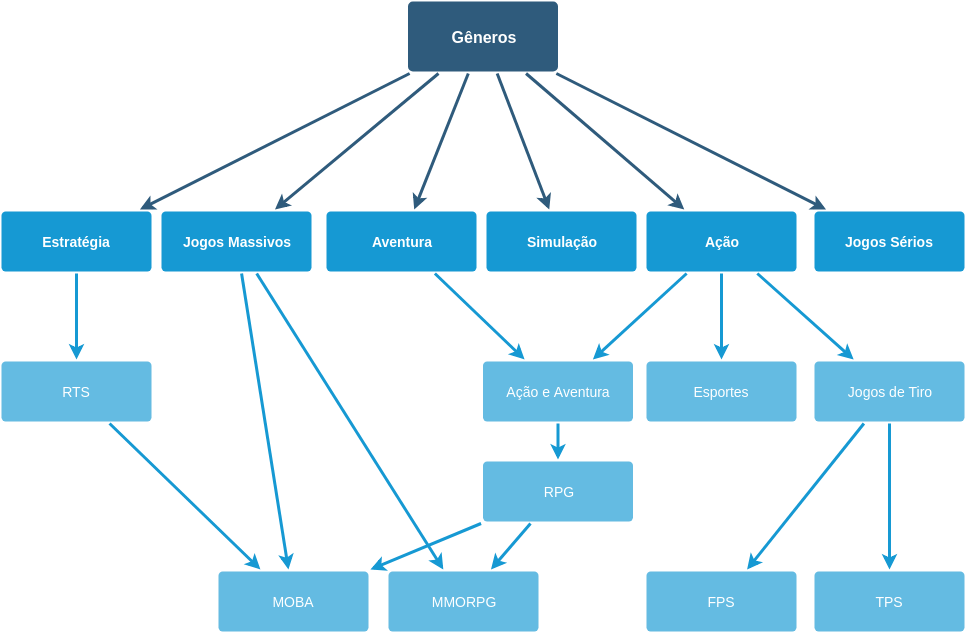
\includegraphics[height=9cm]{img/cap2/generos.png}
\centering

Adaptado de:~\cite{adams_1208533}
\end{figure}



Um gênero de jogo eletrônico é uma categoria específica para agrupar estilos de jogabilidade parecidos.
%
Porém, os gêneros não definem de forma explícita o conteúdo expresso em algum jogo eletrônico, mas sim um desafio comum presente no jogo analisado~\cite{adams_1208533, video_game_technologies}.
%
O contexto breve de cada gênero é (Figura~\ref{fig:generos}):



\begin{itemize}
  \item Estratégia: São focados em uma jogabilidade que exija habilidades de raciocínio e/ou gerenciamento de recurso. Neste gênero, o jogador tem uma boa visualização do mundo, controlando indiretamente as suas tropas disponíveis~\cite{rollings2003andrew}. É comum encontrar jogos que disponibilizam algum modo de competição entre jogadores usando \ac{lan}, \ac{wan} ou \ac{p2p}~\cite{adams_1208533}.
    \begin{itemize}
      \item \ac{rts}: Utiliza as características de um jogo de estratégia, porém esse subgênero indica que as ações dos jogadores são concorrentes. É comum encontrar modos de jogo competitivo utilizando \ac{lan} neste gênero~\cite{adams_1208533}.
    \end{itemize}
  \item \ac{mmo}: Preza pela interação com outros jogadores em um mundo compartilhado~\cite{adams_1208533}. SecondLife\footnote{SecondLife: \url{https://www.secondlife.com/}} é um jogo focado na interação social, com artifícios de comércio e relacionamentos em um mundo fictício criado pela comunidade~\cite{tecmundo_secondlife}. Em grande parte, esses jogos utilizam tecnologia \ac{wan} e \ac{ws}.
    \begin{itemize}
      \item \ac{moba}: Coloca um número fixo de jogadores separados em dois times, no qual o time com maior estratégia de posicionamento e gerenciamento de recursos em equipe ganha a partida. Jogos \ac{moba} perdem algumas características breves do gênero \ac{rpg}, deixando de lado a interpretação e contextualização de um mundo, fixando-se somente em um combate estratégico e momentâneo (distribuído em partidas atômicas) entre as equipes, carregando consigo somente as características de comércio e comunidade dos jogos \ac{mmo}~\cite{adams_1208533}. Tal subgênero é popularmente conhecido pelos títulos Blizzard Dota 2\footnote{Blizzard Dota 2: \url{http://br.dota2.com/}} e Riot League of Legends\footnote{Riot League of Legends: \url{https://br.leagueoflegends.com/pt/}}. O jogo League of Legends obteve 100 milhões de usuários ativos em 2016~\cite{lol_statista}, além de ter um torneio nacional e mundial~\cite{lol_sportv}. É popular nesse subgênero utilizar tecnologias como \ac{lan}, \ac{p2p} e \ac{wan}.
      \item \ac{mmorpg}: Herda características dos gêneros ação e aventura, \ac{rpg}, e \ac{mmo} diretamente. Nesse gênero se faz permitido interações em um mundo na qual outros jogadores também estão jogando, na qual a interação entre outros jogadores (herdado dos jogos \ac{mmo}), com o mundo (herdado dos jogos de ação e aventura) e com objetivos guiados por \ac{npcs} (herdados de jogos \ac{rpg}) se faz como desafio e objetivo do jogo~\cite{adams_1208533}. Um título popular para esse gênero é o jogo Word of WarCraft\footnote{Word of WarCraft: \url{https://worldofwarcraft.com/pt-br/}}. A grande parte dos jogos \ac{mmorpg} utilizam tecnologia \ac{wan}.
    \end{itemize}
  \item Aventura: Caracterizado por desafios envolvendo ações com diversos \ac{npcs} ou com o ambiente para solucionar desafios~\cite{adams_1208533}. A grande parte desses jogos utilizam arquiteturas \ac{wan}, \ac{p2p} ou \ac{lan}.
    \begin{itemize}
      \item Ação e Aventura: Herda características da categoria de Ação e Aventura. O jogador é imerso em um mundo para interagir com o ambiente e com \ac{npcs}, além de se preocupar com a movimentação no cenário~\cite{adams_1208533}. Um título popularmente conhecido desse gênero é a série de jogos nomeada Nintendo The Legend of Zelda\footnote{Nintendo The Legend of Zelda: \url{https://www.zelda.com/}}. É comum nesses jogos encontrar tecnologia \ac{lan} ou \ac{p2p} para modo de jogo cooperativo.
    \end{itemize}
  \item Simulação: Caracterizados por abordar temas da realidade. São comuns jogos de construção e gerenciamento, animais de estimação, vida social e simulação de veículos~\cite{adams_1208533}. A grande parte desses jogos não permite a interação entre os demais jogadores. É popular encontrar serviços como \textit{ranking}, loja e janela de notícias utilizando \ac{ws}.
    \begin{itemize}
      \item Esportes: Trata somente da simulação de esportes, nos quais o(s) time(s) podem ser controlados tanto por uma inteligência artificial quanto por jogadores online~\cite{adams_1208533}. O jogo FIFA\footnote{FIFA: \url{https://www.easports.com/br/fifa}} é um título popular nesse segmento. É comum encontrar tecnologias \ac{p2p} e \ac{lan}.
    \end{itemize}
  \item Ação: Preza pela habilidade de coordenação motora e reflexos do jogador, para tomar uma atitude a fim de passar seus objetivos no cenário. Nesse gênero os objetivos são passar por uma série de desafios que incluam movimentação e posicionamento de outros objetos no cenário~\cite{adams_1208533}. É comum encontrar tecnologias \ac{lan}, \ac{p2p}, \ac{wan} e \ac{ws}.
    \begin{itemize}
      \item Jogos de Tiro: Usa um número finito de armas para executar ações a distância. O posicionamento, movimentação estratégia e mira são fatores de desafio ao jogador nesse gênero~\cite{adams_1208533}. É comum encontrar tecnologias \ac{lan}, \ac{p2p} ou \ac{wan}.
        \begin{itemize}
          \item \ac{fps}: Utiliza o método de gravação conhecido como \ac{pov}. Nesse método, o modo de exibição do mundo é dado como a visão de um personagem do jogo, na qual o jogador tem visão pelo próprio personagem~\cite{video_game_technologies, adams_1208533}. É comum encontrar tecnologias \ac{lan}, \ac{p2p} ou \ac{wan}.
          \item \ac{tps}: Diferente dos jogos \ac{fps}, os jogos \ac{tps} utilizam câmeras soltas no cenário no qual o jogador é visível na cena exibida~\cite{video_game_technologies, adams_1208533}. É comum encontrar tecnologias \ac{lan}, \ac{p2p} ou \ac{wan}.
        \end{itemize}
    \end{itemize}
  \item Jogos sérios: Tem como objetivo transmitir um conteúdo educacional~\cite{video_game_technologies}. O jogo Sherlock Dengue 8~\cite{sherlock_dengue} é um título desenvolvido com o objetivo de conscientizar os problemas e a prevenção da Dengue no Brasil. É comum encontrar tecnologias \ac{lan}, \ac{p2p}, \ac{wan} e \ac{ws}.
\end{itemize}

A árvore de gêneros guia ora aos usuários finais para classificar jogos que lhe agradem ora desenvolvedores a fim de seguir tendências de mercado pelas características do gênero.
%
Dessa forma, encontra-se um padrão nos jogos, na qual também guiam o desenvolvimento das arquiteturas de tais jogos~\cite{video_game_technologies}.

Dentre vários gêneros, alguns utilizam popularmente algumas tecnologias de rede.
%
A Tabela~\ref{tab:comunicacao_genero} indica a correlação de tecnologias de rede comuns nos gêneros, além de trazer a correlação de número de jogadores por gênero de jogo.
%
Essa correlação é importante para identificar as características de jogabilidade referentes a jogabilidade com multijogadores~\cite{video_game_technologies}.


\begin{table}[htb!]
\centering
\caption{Tipos de comunicação e quantia de jogadores populares em gêneros}
\label{tab:comunicacao_genero}
\begin{tabular}{|l|l|l|l|l|l|}
\hline
                & \ac{lan}   & \ac{p2p}   & \ac{wan}            & \ac{ws}  &  Jogadores                                           \\ \hline
ESTRATÉGIA      & \checkmark & \checkmark & \checkmark         &              &   até 10~\cite{eoe3}                              \\ \hline
RTS             & \checkmark &            &                    &              &   até 10~\cite{starcraft2}                        \\ \hline
MOBA            & \checkmark & \checkmark & \checkmark         &              &   até 10~\cite{lol_how_work_games}                \\ \hline
MMO             &            &            & \checkmark         & \checkmark   &   mais que 1000~\cite{runescape_online_users}     \\ \hline
MMORPG          &            &            & \checkmark         & \checkmark   &   mais que 1000~\cite{runescape_online_users}     \\ \hline
AVENTURA        & \checkmark & \checkmark & \checkmark         &              &   até 100~\cite{minecraft}                        \\ \hline
AÇÃO            & \checkmark & \checkmark & \checkmark         & \checkmark   &   até 10~\cite{cuphead}                           \\ \hline
AÇÃO E AVENTURA & \checkmark & \checkmark & \checkmark         &              &   até 10~\cite{cuphead}                           \\ \hline
SIMULAÇÃO       &            &            &                    & \checkmark   &   até 10~\cite{eurotruck2}                        \\ \hline
ESPORTES        & \checkmark & \checkmark &                    &              &   até 10~\cite{fifa2018}                          \\ \hline
FPS             & \checkmark & \checkmark & \checkmark         &              &   até 100~\cite{battlefield3}                     \\ \hline
TPS             & \checkmark & \checkmark & \checkmark         &              &   até 100~\cite{battlefield3}                     \\ \hline
JOGOS SÉRIOS    & \checkmark & \checkmark & \checkmark         & \checkmark   &   até 10~\cite{sherlock_dengue}                   \\ \hline
\end{tabular}

Fonte: O próprio autor.
\end{table}



Dentre todos os jogos, o gênero \ac{mmorpg} é o mais impactado pela quantidade de jogadores\cite{mmo_analytic}, visível na Tabela~\ref{tab:comunicacao_genero}.
%
Nesse sentido, as arquiteturas do serviço e cliente se tornam um ponto crítico no desenvolvimento a fim de suportar a carga necessária ao desenho do jogo.
%
Por esse motivo, a escolha por abordar o gênero \ac{mmorpg} se torna interessante do ponto de vista computacional, a fim de analisar o comportamento e consumo de jogos \ac{mmorpg}, visando obter características destas arquiteturas.



\section{\ac{mmorpg}}
\label{sec:mmorpg}



Jogos \ac{mmorpg} são utilizados como negócio viável e lucrativo, sendo que a experiência de jogabilidade na qual o usuário final será submetido é um fator crítico para o sucesso.
%
O mercado de jogos \ac{mmorpg} vem crescendo desde 2012~\cite{new_york_times}, sendo no ano de 2017 um dos mais lucrativos~\cite{statista_2018_mmo}.
%
A projeção deste mercado para 2018 é de mais de 30 bilhões de dólares americanos com esta categoria de jogos~\cite{statista_2018}, porém foi ultrapassado no ano de 2017 com 30,7 bilhões de dólares~\cite{statista_2018_mmo}.



\ac{mmorpg} são jogos de interpretação de papéis massivos, originados dos gêneros \ac{rpg}.
%
A principal característica desse estilo de jogo é a comunicação e representação virtual de um mundo fantasia no qual cada jogador pode interagir com objetos virtuais compartilhados ou tomar ações sobre outros jogadores em tempo real, tendo como principais objetivos a resolução de problemas conforme a sua regra de \textit{design}, o desenvolvimento do personagem e a interação entre os jogadores\cite{video_game_technologies}.



Um jogo \ac{mmorpg} é arquitetado em duas partes~\cite{mmo_analytic}:
\begin{itemize}
  \item \textbf{Cliente}: Aplicação que realiza as requisições com a interface do serviço, exibindo o estado de jogo de forma imersiva ao jogador. Este tema é melhor abordado na Seção \ref{sec:cliente}.
  \item \textbf{Servidor}: Conjunto de computadores que recebe as requisições do cliente a fim de ser processadas pelo Serviço.
  \item \textbf{Serviço}: Implementa as regras de negócio e requisitos do jogo. O serviço disponibiliza uma interface com ações possíveis ao cliente sobre algum protocolo de rede. Este tema é melhor abordado na Seção~\ref{sec:microsservicos}.
\end{itemize}

Jogos \ac{mmorpg} trabalham como serviço. Por este motivo o modelo de negócios de tais jogos, do ponto de vista de redes de computador, são suscetíveis a perda financeira em casos de negação de serviço~\cite{1417630}.
%
A maioria dos jogos \ac{mmorpg} disponíveis no mercado estão implementados sobre uma arquitetura que executa sobre diversos servidores~\cite{stephenclarkewillson2017}, nos quais o desempenho destes servidores influencia tanto na experiência de jogabilidade do usuário final, quanto no custo de manutenção destes serviços~\cite{1417630}.
%
Por sua vez, o Cliente é implementado em algum ambiente convencional a jogos, como motores gráficos, bibliotecas gráficas ou sobre alguma outra plataforma, como web.
%
Nesse sentido, torna-se necessário descrever as características de jogabilidade de jogos \ac{mmorpg} a fim de melhor compreender o funcionamento da arquitetura de um cliente e de um serviço para jogos \ac{mmorpg}.



\section{Jogabilidade de jogos MMORPG}
\label{sec:jogabilidade}



É comum em jogos \ac{mmorpg} ter sistemas com funcionalidades parecidas.
%
Por esse motivo é fácil identificar os sistemas em jogos do mercado após a compreensão dos sistemas identificados.
%
Deste modo, torna-se necessário definir algumas funcionalidades básicas que estão dentro do contexto de jogabilidade de jogos \ac{mmorpg} para melhor compreensão de sua arquitetura em seções futuras.


O sistema de autenticação é o sistema que geralmente inicia o cliente de algum jogo \ac{mmorpg}~\cite{albion_online_unite, matthiasrudy2011}.
%
Este sistema é implementado via protocolo web, a fim de disponibilizar um código para validar todas as futuras ações da seção do usuário.
%
Ele pode ser visualizado de forma macro na Figura~\ref{fig:autenticacao}.

\begin{figure}[htb!]
\caption{Sistema de autenticação para jogos}
\label{fig:autenticacao}
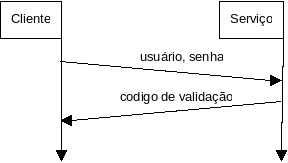
\includegraphics[height=3cm]{img/cap2/autenticacao.png}
\centering

Fonte: Adaptado de ~\cite{LeckyThompson2008Nov}
\end{figure}


O sistema de autenticação visualizado na Figura~\ref{fig:autenticacao} é o principal, porém não o único.
%
O jogo Realm of the Mad God\footnote{Realm of the Mad God: \url{https://www.realmofthemadgod.com/}} é um exemplo na qual não exige autenticação do usuário, entretanto ele não armazena o progresso do jogador caso o jogador não efetue a autenticação.


Esse método de autenticação é definido pela RFC7519~\cite{rfc7519}, com a tecnologia \ac{jwt}.
%
O código de validação repassado é auditorado em qualquer serviço pertencente ao jogo, visto que ele foi assinado pelo sistema de autenticação do serviço~\cite{Ikem2018May}.


Após a autenticação, é comum existir um sistema para seleção de personagem, caso o jogo seja desenhado com este objetivo.
%
Efetuada a seleção ou criação de um personagem, este será imerso no mundo compartilhado do jogo com os demais jogadores~\cite{matthiasrudy2011}.
%
Nos jogos \ac{mmorpg} é comum a restrição da visão do personagem (Figura~\ref{fig:proximidade}), ora pelas características de jogabilidade do gênero \ac{mmorpg} ora por motivos de desempenho e otimização.
%
Como o jogador não precisa obter dados de regiões que não estão em sua área de interesse, não há necessidade da transmissão de informações dos objetos que estão fora desse contexto~\cite{albion_online_unite}.

\begin{figure}[htb!]
\caption{Área de interesse com base na proximidade de um jogador}
\label{fig:proximidade}
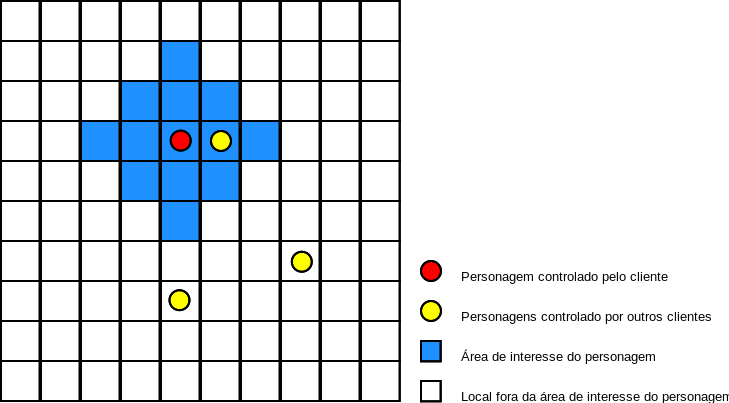
\includegraphics[height=3.8cm]{img/cap2/proximidade.png}
\centering

Fonte:~\cite{albion_online_unite}
\end{figure}


Esse caso pode ser visualizado na Figura~\ref{fig:proximidade}, na qual o personagem selecionado (destacado em vermelho) tem uma área de interesse de baixa distância e uma área de interesse de longa distância~\cite{albion_online_unite}, sendo que o jogador não tem informações dos demais objetos e jogadores fora de sua área de interesse.
%
Esta característica impede trapaças (visto que o cliente não tem informações que só estão contidas no serviço) e reduz a frequência de atualização a cada cliente~\cite{albion_online_unite}.


Após o jogador estar com o controle do personagem no ambiente, é comum em tais jogos que ele possa realizar determinadas ações.
%
Nesse sentido, algumas ações comuns dentro do ambiente de um jogo \ac{mmorpg}~\cite{mmorpg_culture}:

\begin{itemize}
  \item Enviar e receber mensagem no chat;
  \item Mover-se pelo ambiente;
  \item Interagir com outros jogadores, \ac{npcs} ou objetos fixos do ambiente; e
  \item Obter itens do ambiente.
\end{itemize}



O envio e recepção de mensagens do chat é dado com o contexto do posicionamento do personagem~\cite{albion_online_unite}, visível na Figura~\ref{fig:chat}.
%
Somente outros personagens dentro de uma distância podem receber alguma mensagem emitida pelo jogador $P_n$.

\begin{figure}[htb!]
\caption{Chat baseado em contexto de posicionamento, utilizando Distância Euclidiana}
\label{fig:chat}
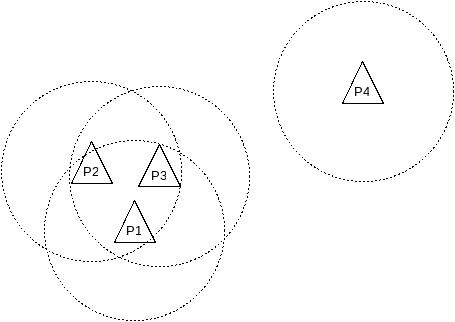
\includegraphics[height=8cm]{img/cap2/chat.png}
\centering

Fonte: Adaptado de ~\cite{albion_online_unite}
\end{figure}

Essa distância (Figura~\ref{fig:chat}) pode ser calculada utilizando Distância Euclidiana~\cite{Deza2009Aug}, na qual a distância entre dois personagens podem ser calculadas pela equação $d(p, q) = \sqrt{\sum_{i=1}^{n}(q_i - p_i)^2}$.
%
Para diminuir a complexidade das comparações, a fim de decidir quais personagens $P_n$ devem receber a mensagem, é comum utilizar técnicas de divisão de área utilizando algoritmos como \textit{Quadtree} ou \textit{Octree}~\cite{Lengyel2011Jun}, subdividindo os quadrantes de uma região do ambiente do jogo a fim de facilitar a consulta de quais personagens estão em determinada área deste ambiente.


Nesse sentido, a Figura~\ref{fig:chat} mostra a interseção entre o raio de quatro personagens.
%
Nesse exemplo, mostra-se visível que a as mensagens de $P_1$ devem ser visíveis a $P_2$ e $P_3$, mas não a $P_4$, caso seja utilizado a Distância Euclidiana como regra de distância.



O sistema de movimento pelo ambiente do jogo possibilita que cada jogador movimente o seu personagem pelo ambiente a fim de explorá-lo.
%
Dessa maneira, este é um sistema crítico para um jogo \ac{mmorpg}, visto que o posicionamento de objetos serão utilizados para diversas consultas de proximidade, além de necessitar uma frequência de atualização contante pela qualidade da jogabilidade~\cite{albion_online_unite}.


\begin{figure}[htb!]
\caption{Personagens e os seus pontos de destino}
\label{fig:walk}
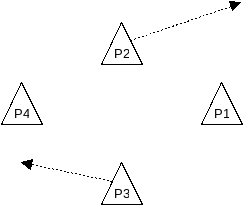
\includegraphics[height=4cm]{img/cap2/walk.png}
\centering

Fonte: O próprio autor.
\end{figure}



A interação com o ambiente, itens, \ac{npcs} e outros jogadores também são afetados pela área de interesse, na qual o personagem terá um raio limitante para cada tipo de interação no ambiente.
%
Um exemplo de ambiente com personagens ($P_1$ e $P_2$), objetos ($O_1$) e \ac{npcs} (NPC somente) pode ser visualizado na Figura~\ref{fig:obj_e_npc1}~\cite{albion_online_unite}.

\begin{figure}[htb!]
\caption{Personagens, objetos e NPCs em no ambiente}
\label{fig:obj_e_npc1}
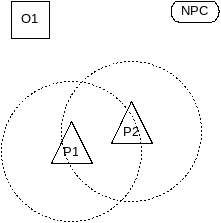
\includegraphics[height=4cm]{img/cap2/obj_e_npc1.png}
\centering

Fonte: O próprio autor.
\end{figure}



Essas operações precisam de desempenho para não causar frustração ao jogador final~\cite{7008965}.
%
Nesse sentido, torna-se necessário conhecer os problemas computacionais conhecidos com relação aos serviços de jogos \ac{mmorpg}.



\section{Problemas em jogos MMORPG}
\label{sec:problemas}

Uma métrica popular para mensurar o desempenho de um serviço \ac{mmorpg} é o número de conexões~\cite{1417630} simultâneas suportadas.
%
Em geral, caso o serviço ultrapasse o limite para o qual este foi projetado, diversas falhas de conexão, problemas de lentidão ou dessincronização com o cliente podem ocorrer.
%
Neste contexto, as ocorrências comuns são~\cite{1417630}:

\begin{itemize}
  \item \textbf{Longo tempo de resposta aos clientes}: implica em uma qualidade insatisfatória de jogabilidade ao usuário ou até mesmo impossibilitando o uso do serviço.
  \item \textbf{Dessincronização com os clientes}: realiza reversão na aplicação. Reversão é definida pela situação na qual uma requisição é solicitada ao servidor, um pré-processamento aparente é executado e essa requisição é negada, sendo necessário desfazer o pré-processamento aparente realizado ao cliente.
  \item \textbf{Problemas internos ao serviço}:  podem estar relacionados a diversos outros erros internos de implementação ou a capacidade de recurso computacional (\textit{e.g.,} sobrecarga no banco de dados, gerenciamento lento do espaço ou inconsistências dentro do jogo perante a regra de negócios).
  \item \textbf{Falha de conexão entre o cliente e o serviço}: causa a negação de serviço ao usuário final.
\end{itemize}

Existem algumas causas comuns para essas as ocorrências descritas~\cite{1417630}:

\begin{itemize}
  \item \textbf{Baixo poder computacional do servidor}: poder computacional baixo para a qualidade de experiência de jogabilidade do usuário final desejada.
  \item \textbf{Complexidade de algoritmos}: o serviço usa algoritmos de alta complexidade ou regras de negócios que demandam por um algoritmo complexo.
  \item \textbf{Limitado pela própria arquitetura}: está limitado diretamente pelo número de conexões, não suportando a carga recebida.
  \item \textbf{Limitado pela rede}: a quantidade de requisições não é suportada pelo meio físico na qual a arquitetura está implantada.
\end{itemize}

Tais ocorrências estão diretamente correlacionadas a carga a qual tais serviços estão submetidos e podem ser amenizadas utilizando técnicas de provisionamento de recursos e balanceamento de carga~\cite{1417630}, mas não suficiente para eliminar tais ocorrências.

A área de desenvolvimento web compartilha várias ocorrências comuns geradas por sobrecarga do serviço~\cite{7830692}.
%
Em desenvolvimento web é comum utilizar a abordagem de microsserviços para resolver o problema de sobrecarga, modularizando o  funcionamento em módulos menores.
%
Da mesma forma, faz sentido modularizar um serviço \ac{mmorpg} em microsserviços para suportar cargas maiores e diminuir o custo de manutenção~\cite{7515686}.



Do ponto de vista da arquitetura de computadores, as operações existentes em um jogo \ac{mmorpg} seguem um padrão de interação com o mundo, criar, excluir ou manipular objetos deste mundo.
%
Para suprir o desenvolvimento de tais sistemas, se faz necessário compreender os padrões de desenvolvimento de tais arquiteturas na qual suprem as operações básicas de interação com o mundo.



\subsection{Arquitetura de Clientes MMORPG}
\label{sec:cliente}



A arquitetura de um cliente \ac{mmorpg} é um aspecto fundamental, mas não único, para o sucesso de um jogo deste gênero.
%
O seu funcionamento é totalmente visível ao usuário final e tem o principal objetivo de exibir o estado do mundo de forma gráfica ao usuário~\cite{albion_online_unite}.
%
Um exemplo de cliente \ac{mmorpg} é o jogo Sandbox-Interactive Albion\footnote{Sandbox-Interactive Albion: \url{https://albiononline.com/en/home}}, que pode ser visualizado na Figura~\ref{fig:cliente_albion}.



\begin{figure}[htb!]
\caption{Exemplo de Cliente MMORPG (Sandbox-Interactive Albion).}
\label{fig:cliente_albion}
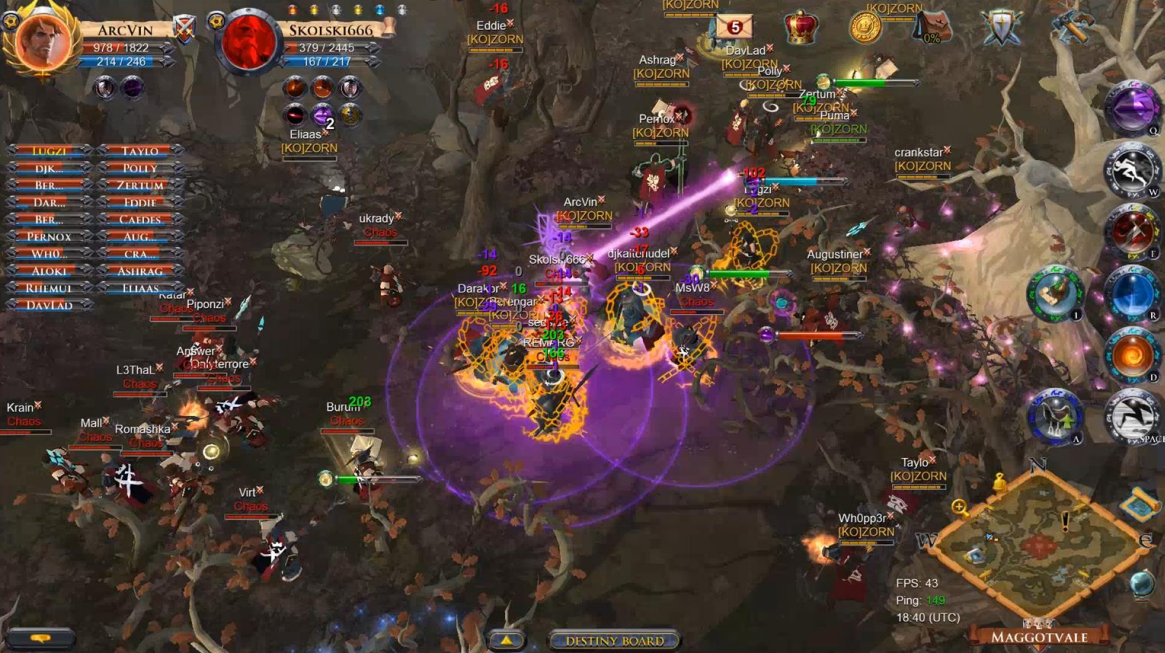
\includegraphics[height=8cm]{img/cap2/cliente_albion.png}
\centering

Fonte:~\cite{albion_online_unite}
\end{figure}


Do ponto de vista de computação gráfica, um cenário 3D pode ser visualizado como uma árvore.
%
Utilizar árvores para descrever um cenário ajuda tanto no formado de armazenamento em disco para leitura facilitada (\textit{e.g.}, \ac{json}, \ac{xml}, etc.), operações de inserção e exclusão, organização do projeto e redução da complexidade utilizando transformações lineares em sistemas gráficos como \textit{OpenGL} e \textit{DirectX}~\cite{Lengyel2011Jun}.
%
Esse modelo é amplamente utilizado em motores gráficos, na qual pode ser encontrado em motores gráficos populares como \textit{Godot}, \textit{Unity3D} e \textit{Unreal 3}.
%
A Figura~\ref{fig:scene_tree} ilustra um exemplo, na qual exibe a árvore de um cenário na \ac{ide} do motor gráfico \textit{Godot}.



\begin{figure}[htb!]
\caption{\textit{Scene tree view} no motor gráfico Godot}.
\label{fig:scene_tree}
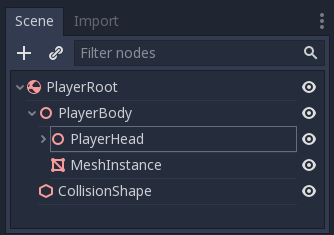
\includegraphics[height=5cm]{img/cap2/scene_tree.png}
\centering

Fonte: O próprio autor.
\end{figure}



Dentro dessa árvore, cada nodo tem uma funcionalidade específica.
%
Essas funcionalidades são específicas a cada motor gráfico, podendo existir nodos específicos a física, renderização ou controles~\cite{godot_docs}.
%
Em um jogo \ac{mmorpg}, o serviço será responsável por enviar atualizações dos parâmetros aos nodos frequentemente e o cliente será responsável por realizar chamadas remotas a fim de descrever as ações a qual o jogador aplicou sobre seu personagem~\cite{photon_engine}.


Do ponto de vista da rede de computadores, a arquitetura de um cliente de jogo \ac{mmorpg} deve suportar consultas e chamadas de métodos remotos em um serviço~\cite{albion_online_unite}.
%
Um cliente para um jogo \ac{mmorpg} pode seguir o estilo de arquitetura \ac{rest}, porém não obrigatoriamente sobre o protocolo \ac{http}, mas sim usando algum protocolo \ac{rpc} sobre o protocolo \ac{tcp} ou \ac{udp}~\cite{albion_online_unite, stephenclarkewillson2017}.
%
Essa comunicação é realizada pelo módulo \textit{Network}, presente em um cliente \ac{mmorpg}.


O módulo de \textit{Network} implementado em um cliente de jogo \ac{mmorpg} é responsável por realizar as requisições \ac{rpc} conforme as ações solicitadas pelo jogador ao serviço, além de aplicar os parâmetros na \textit{Scene Tree} ou chamar métodos remotos no cliente por ordens do serviço.
%
E módulo possui uma \textit{Thread} dedicada ao seu funcionamento~\cite{albion_online_unite}.
%
Ele pode ser observado na Figura~\ref{fig:gateway}.


\begin{figure}[htb!]
\caption{Modelo de um cliente genérico.}
\label{fig:gateway}
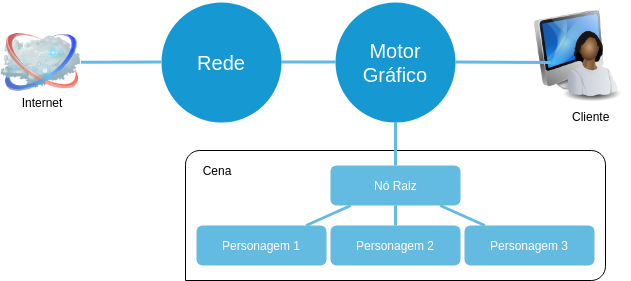
\includegraphics[height=5cm]{img/cap2/cliente.png}
\centering

Adaptado de:~\cite{507915, faber}
\end{figure}


A Figura~\ref{fig:gateway} refere-se a uma visão macro de um cliente \ac{mmorpg}.
%
Na Figura~\ref{fig:gateway} é possível ver o ator \textit{player} o qual pode executar ações sobre seu personagem por meio da \textit{engine}.
%
Por sua vez, existe uma entrada de dados a mais comparado a esquemas de jogos \textit{offline}.
%
Neste caso, o módulo \textit{Network} será também uma entrada de dados, a qual poderá manipular a cena do motor gráfico~\cite{faber}.



Para facilitar o desenvolvimento, a aplicação de cliente é dividida em diversos módulos, entretanto são relevantes ao atual trabalho~\cite{albion_online_unite}:



\begin{itemize}
  \item \textbf{Engine:} É o conjunto que aplicará regras sobre os objetos na \textit{Scene Tree}, receberá entradas do usuário e exibirá a \textit{Scene Tree} de forma imersiva. Unity3D\footnote{Unity3D: \url{https://www.unity3d.com}} e GodotEngine\footnote{GodotEngine: \url{https://www.godotengine.org}} são exemplos de \textit{engines}.
  \item \textbf{Network:} É o módulo responsável pela comunicação entre o serviço e o cliente, a fim de requisitar chamadas de métodos ou obter informações do servidor para sincronizar os estados de jogo.
\end{itemize}



Utilizando esses dois módulos é possível sincronizar os estados de jogo e exibi-los ao jogador.
%
Entretanto, faz-se necessário compreender o funcionamento do serviço a fim de escolher um protocolo padrão para essa sincronização.



\subsection{Arquitetura de Microsserviços}
\label{sec:microsservicos}



Entende-se por microsserviço, aplicações que executam operações menores de um macrosserviço, da melhor forma possível~\cite{stephenclarkewillson2017, Newman2015Feb}.
%
O objetivo de uma arquitetura de microsserviços é funcionar separadamente de forma autônoma, contendo baixo acoplamento~\cite{Newman2015Feb}.
%
Seu funcionamento deve ser desenhado para permitir alinhamentos de alta coesão e baixo acoplamento entre os demais microsserviços existentes em um macrosserviço~\cite{8169955}.



Arquiteturas de microsserviços iniciam uma nova linha de desenvolvimento de aplicações preparadas para executar sobre nuvens computacionais, promovendo maior flexibilidade, escalabilidade, gerenciamento e desempenho, sendo a principal escolha de arquitetura de grandes empresas como Amazon, Netflix e LinkedIn~\cite{7830692,7515686}.
%
Um microsserviço é definido pelas seguintes características~\cite{8169955}:



\begin{itemize}
  \item Deve possibilitar a implementação como uma peça individual do macrosserviço.
  \item Deve funcionar individualmente.
  \item Cada serviço deve ter uma interface. Essa interface deve ser o suficiente para utilizar o microsserviço.
  \item A interface deve estar disponível na rede para chamada de processamento remoto ou consulta de dados.
  \item O serviço pode ser utilizado por qualquer linguagem de programação e/ou plataforma.
  \item O serviço deve executar com as dependências mínimas.
  \item Ao agregar vários microsserviços, o macrosserviço resultante poderá prover funcionalidades complexas.
\end{itemize}



O microsserviço deverá ser uma entidade separada.
%
A entidade deve ser implantada sobre um sistema isolado (\textit{e.g.,} Docker~\footnote{Docker:~\url{https://www.docker.com/}}, \acp{vm}, \textit{etc.}).
%
Toda a comunicação entre os microsserviços de um macrosserviço será executada sobre a rede, a fim de reforçar a separação entre cada serviço.
%
As chamadas pela rede com o cliente ou entre os microsserviços será executada através de uma \ac{api}, permitindo a liberdade de tecnologia em que cada um será implementado~\cite{Newman2015Feb}.
%
Isso permite que o sistema suporte tecnologias distintas que melhor resolvam os problemas relacionados ao contexto deste microsserviço.
%
Isso pode ser visualizado na Figura~\ref{fig:microsservicos_tecnologias}.



\begin{figure}[htb!]
\caption{Microsserviços podem ter diferentes tecnologias}
\label{fig:microsservicos_tecnologias}
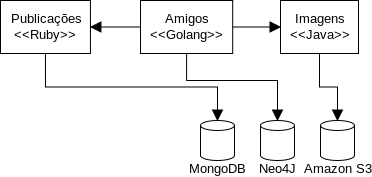
\includegraphics[height=4cm]{img/cap2/microsservicos_tecnologias.png}
\centering

Adaptado de:~\cite{Newman2015Feb}
\end{figure}


Uma arquitetura de microsserviços é escalável, como visível na Figura~\ref{fig:microsservicos_escalabilidade}.
%
A arquitetura permite o aumento do número de microsserviços sob demanda para suprir a necessidade de escalabilidade.
%
Este modelo computacional obtém maior desempenho, principalmente se executar sobre plataformas de computação elástica, na qual o orquestrador do macrosserviço pode aumentar o número de instâncias conforme a necessidade de requisições~\cite{Nadareishvili2016Aug}.



\begin{figure}[htb!]
\caption{Microsserviços são escaláveis}
\label{fig:microsservicos_escalabilidade}
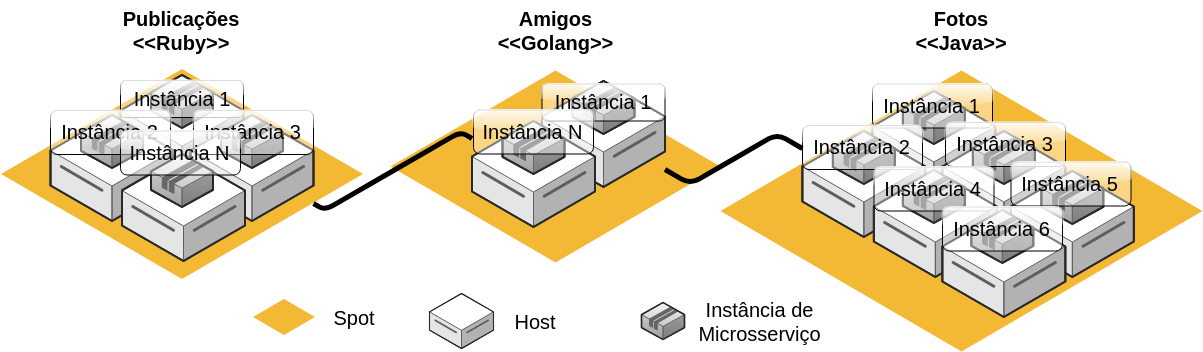
\includegraphics[height=5cm]{img/cap2/microsservicos_escalabilidade.png}
\centering

Adaptado de:~\cite{Newman2015Feb}
\end{figure}



Microsserviços desenvolvidos para web utilizam arquitetura \ac{rest} baseado sobre o protocolo \ac{http}.
%
É uma boa prática utilizar o corpo com conteúdo da requisição e resposta no formato \ac{json} nas chamadas a uma \ac{api} de microsserviço web~\cite{Nadareishvili2016Aug}.
%
Entretanto, não é uma prática comum para um serviço \ac{mmorpg} utilizar o protocolo \ac{http} pela sua elevada carga administrativa na requisição~\cite{1417630}.
%
Por esse motivo, torna-se relevante compreender a composição de uma arquitetura com microsserviços para \ac{mmorpg}, comparado-a a microsserviços web.



\subsection{Microsserviços para jogos \ac{mmorpg}}
\label{sec:arquiteturas}



A fim de otimizar o custo operacional das arquiteturas de microsserviços de jogos \ac{mmorpg}, é incomum a utilização de protocolos \textit{Web} em tais arquiteturas.
%
Por esse motivo, a seção atual mostrará o funcionamento básico do protocolo \ac{rpc} e a sua utilização para atualização dos parâmetros na \textit{Scene Tree} e o modelo \ac{rest}~\cite{albion_online_unite}.



Em engenharia de software, é comum a utilização de arquiteturas \ac{mvc} a fim de organizar o código fonte e prover agilidade de desenvolvimento~\cite{Chadwick2012Oct, LeckyThompson2008Nov}.
%
A separação de um serviço \ac{mmorpg} pode ser dada seguindo este padrão de projeto, dividindo-se em três camadas~\cite{5718337}:


\begin{enumerate}
  \item \textit{Model}: Representa qualquer dado presente no jogo (\textit{e.g.,} itens, personagens, \ac{npcs}, objetivos, etc.).
  \item \textit{View}: Representa o modo a qual estes dados serão exibidos, do ponto de vista de redes (\textit{e.g.,} O mapa será exibido somente na área de interesse do jogador, e esta redução de contexto pode ser aplicada na visualização).
  \item \textit{Controller}: Representa as operações sobre modelos que serão requiridos pelos jogadores (\textit{e.g.,} andar, pegar item, interagir com \ac{npcs}, etc.).
\end{enumerate}



Dentro de um \textit{Controller} é implementado operações a qual o cliente pode requirir através de chamadas \ac{rpc} a fim de manipular \textit{Models} da aplicação.
%
Esses métodos padrões seguem o protocolo \ac{crud}, contendo quatro métodos principais para complementar as consultas sobre os \textit{Models}~\cite{Chadwick2012Oct, LeckyThompson2008Nov}:



\begin{enumerate}
  \item \textit{Create}: Representa a criação de um novo objeto no banco.
  \item \textit{Update}: Representa a atualização de um objeto no banco.
  \item \textit{Delete}: Representa a exclusão de um objeto no banco.
  \item \textit{Read}: Representa a consulta sobre este objeto no banco.
\end{enumerate}



Para o padrão \ac{crud}, faz-se necessário que os métodos \textit{Read}, \textit{Update} e \textit{Delete} repassem o parâmetro de identificação do objeto a ser consultado~\cite{LeckyThompson2008Nov}.
%
Outros argumentos necessários nos métodos \textit{Create} e \textit{Update} são os atributos do objeto, além do seu retorno ser um valor booleano representando se a operação foi bem sucedida~\cite{Chadwick2012Oct, LeckyThompson2008Nov}.
%
Entretanto, outros métodos mais apropriados ao funcionamento de um \textit{Controller} podem existir.
%
Como exemplo, pode-se visualizar uma interface \ac{crud} na Figura~\ref{fig:crud}.



\begin{figure}[htb!]
\caption{Cliente pode realizar requisições \ac{crud} ao serviço.}
\label{fig:crud}
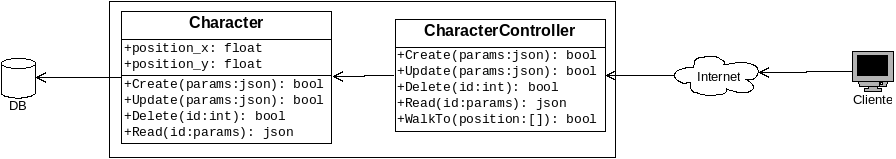
\includegraphics[height=2.5cm]{img/cap2/crud.png}
\centering

Fonte: Adaptado de~\cite{albion_online_unite}.
\end{figure}



Essas operações são executadas utilizando protocolo \ac{rpc}~\cite{albion_online_unite}.
%
As requisições de métodos remotos são realizadas entre dois processos distintos, a fim de gerar uma computação distribuída~\cite{rpc}.
%
Entretanto, a base do protocolo não é legível como em servidores web que utilizam \ac{json} para transmissão de estrutura de dados, mas sim uma codificação binária nomeado \ac{xdr}~\cite{xdr}.

\begin{figure}[htb!]
\caption{Diagrama de requisições entre serviço e cliente com operações \ac{crud} e \ac{rpc} em uma arquitetura monolítico.}
\label{fig:network_crud_rpc}
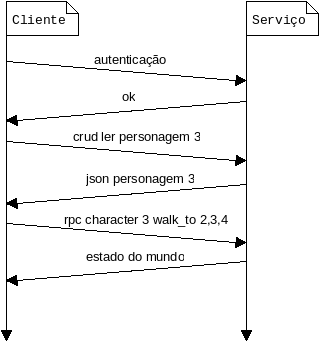
\includegraphics[height=6.5cm]{img/cap2/network_rpc_crud.png}
\centering

Fonte: Adaptado de~\cite{LeckyThompson2008Nov}
\end{figure}



Uma técnica comum em jogos é a compressão de pacotes utilizando mapeamento \textit{hash} de bytes~\cite{LeckyThompson2008Nov}.
%
Tanto o cliente quanto o serviço precisam ter a mesma estrutura de dados.
%
Dessa forma, é possível trocar o nome das funções solicitadas em \ac{rpc} por poucos bytes para transitar na rede.
%
Já para operações \ac{crud}, pode-se utilizar tanto requisições sobre o protocolo \ac{http} ou sobre um protocolo otimizado sobre \ac{tcp} dependendo da necessidade de desempenho~\cite{LeckyThompson2008Nov}.

Como relatado na Seção~\ref{sec:microsservicos}, uma arquitetura de microsserviços permite múltiplas tecnologias, pois a comunicação entre todos os elementos de um microsserviço será pela rede.
%
Por esse motivo, é possível utilizar um serviço web para realizar operações \ac{crud} e um serviço dedicado para realizar operações \ac{rpc}.
%
Essa arquitetura pode ser melhor visualizada na Figura~\ref{fig:network_crud_rpc_micro}.



\begin{figure}[htb!]
\caption{Diagrama de requisições entre serviço e cliente com operações \ac{crud} e \ac{rpc} em uma arquitetura de microsserviços.}
\label{fig:network_crud_rpc_micro}
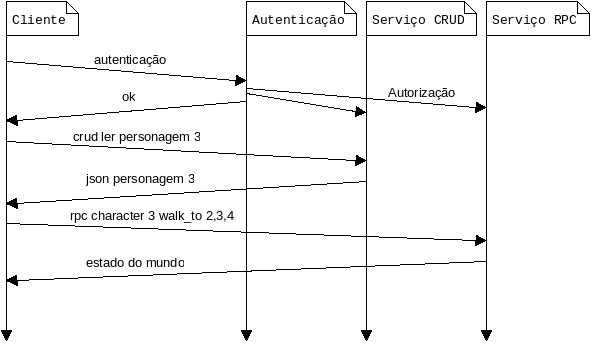
\includegraphics[height=6.5cm]{img/cap2/network_rpc_crud_micro.png}
\centering

Fonte: O próprio autor.
\end{figure}



Como resultado da integração entre Cliente, Serviço e Motor Gráfico, o resultado final obtido é descrito pelo diagrama presente na Figura~\ref{fig:integracao_unity_albion}.
%
Tal integração está presente no jogo Sandbox-Interactive Albion\footnote{Sandbox-Interactive Albion: \url{https://albiononline.com/en/home}}~\cite{albion_online_unite}.
%
Percebe-se neste contexto que o jogo deverá funcionar sem o motor gráfico, do ponto de vista de redes e estrutura de dados~\cite{albion_online_unite}.


\begin{figure}[htb!]
\caption{Diagrama de integração entre Cliente e Serviço, considerando a \textit{engine} Unity3D.}
\label{fig:integracao_unity_albion}
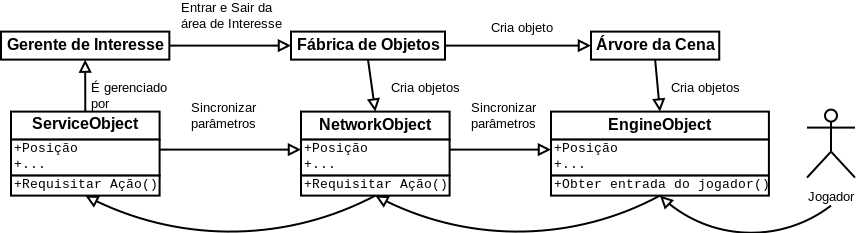
\includegraphics[height=6.5cm]{img/cap2/integracao_unity_albion.png}
\centering

Fonte:~\cite{albion_online_unite}
\end{figure}

A Figura~\ref{fig:integracao_unity_albion} demonstra a separação da camada de renderização de objetos da árvore da cena, a camada de integração com o cliente e serviço (descrito anteriormente como módulo \textit{Network}) e o serviço.
%
Nesse sentido, a alteração entre clientes e serviços facilita um sistema de teste de carga e busca de erros automatizado, facilitando a manutenção e desenvolvimento incremental do serviço~\cite{albion_online_unite}.

Utilizando estas características, alguns padrões tornam-se populares nessas arquiteturas.
%
Torna-se de interesse a este trabalho realizar um levantamento de algumas arquiteturas comuns em jogos massivos.



\subsection{Arquitetura elaborada por Rudy}




A arquitetura Rudy~\cite{matthiasrudy2011} tem como objetivo criar múltiplos mundos isolados, na qual cada microsserviço será responsável por um ambiente a qual não compartilha dados com os demais ambientes.
%
Esta arquitetura pode ser visualizada na Figura~\ref{full_rudy}.

\begin{figure}[htb!]
  \caption{Arquitetura Rudy completa.}
  \label{full_rudy}
  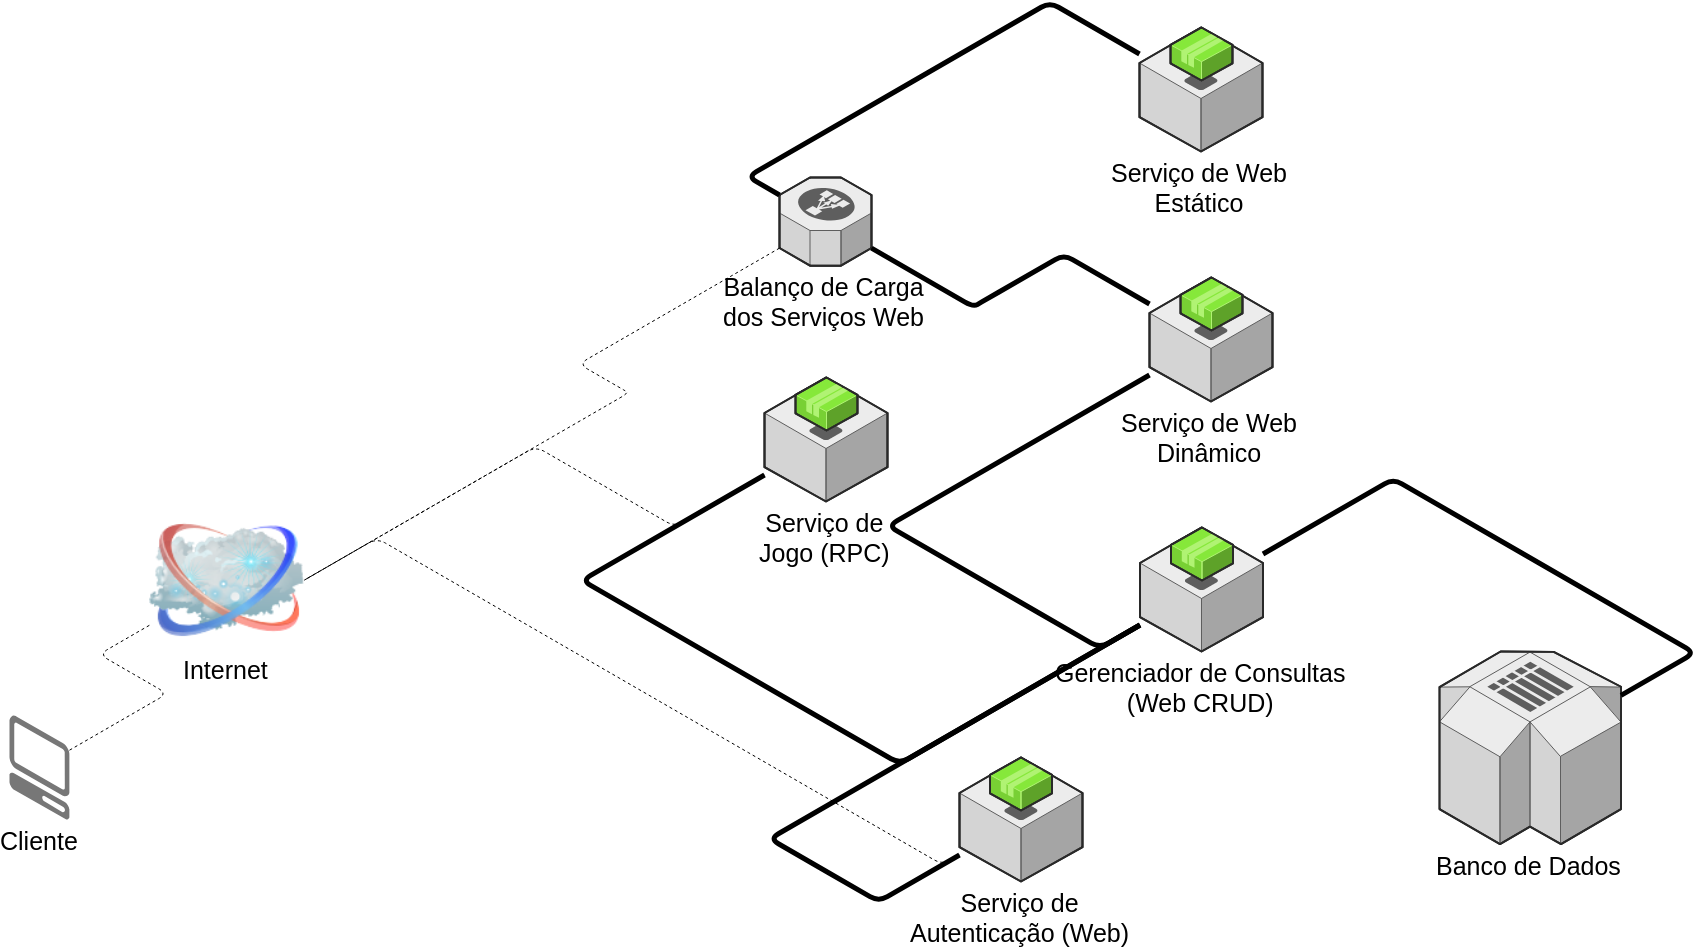
\includegraphics[height=5.5cm]{arquiteturas/full_rudy.png}
  \centering

  Fonte:~\cite{matthiasrudy2011}.
\end{figure}

Ao todos são 6 microsserviços distintos na arquitetura Rudy para o seu funcionamento, utilizando um microsserviço de pagamento necessário para regra de negócios como exibido na Figura~\ref{full_rudy}.
%
Os microsserviços que compõem a arquitetura são definidos pelas suas seguintes responsabilidades~\cite{matthiasrudy2011}:
\cite{matthiasrudy2011}:

\begin{enumerate}
  \item \textbf{Serviço web estático}: Armazena documentos estáticos para o serviço web (\textit{e.g., }imagens, executáveis do jogo, páginas web fixas, etc).
  \item \textbf{Serviço web dinâmico}: Sistema web para cadastro de contas, guias, informações sobre atualizações, compras e demais demanda de páginas dinâmicas.
  \item \textbf{Balanço de carga web}: Realiza a distribuição de carga sobre o \textit{Serviço web estático} e o \textit{Serviço web dinâmico}.
  \item \textbf{Serviço de Jogo}: Gerencia um mundo inteiro, em um único serviço. Esta abordagem segrega os jogadores em diversos mundos, contendo 1050 jogadores simultâneos por serviço. Este serviço opera sobre o protocolo \ac{rpc}.
  \item \textbf{Serviço de Autenticação}: Gerencia a autenticação das conexões ao \textit{Serviço de jogo}.
  \item \textbf{Gerenciador de Consultas}: Realiza consultas em memória e disco, utilizando vários bancos de dados diferentes, simulando o uso de banco de dados distribuídos, algo complexo de ser implementado utilizando banco de dados SQL (\textit{e.g.,} PostgreSQL\footnote{PostgreSQL: \url{https://www.postgresql.org}}, MySQL\footnote{MySQL: \url{https://www.mysql.com/}}, etc).
\end{enumerate}


No contexto do atual trabalho, o serviço de pagamento será ignorado, visto que ele não serve para o funcionamento básico do serviço.
%
Dentre todos os microsserviços, o usuário só tem acesso ao serviço de balanço de carga pelo protocolo \ac{http} e o serviço de jogo sobre o protocolo \ac{rpc}, tendo os demais serviços protegidos por um \textit{firewall}~\cite{matthiasrudy2011}.
%
A proteção do firewall é aplicada no serviço de pagamento e no ponto de acesso ao serviço, podendo ser vizualizada na Figura~\ref{full_rudy_fw}.

\begin{figure}[htb!]
  \caption{Arquitetura Rudy completa.}
  \label{full_rudy_fw}
  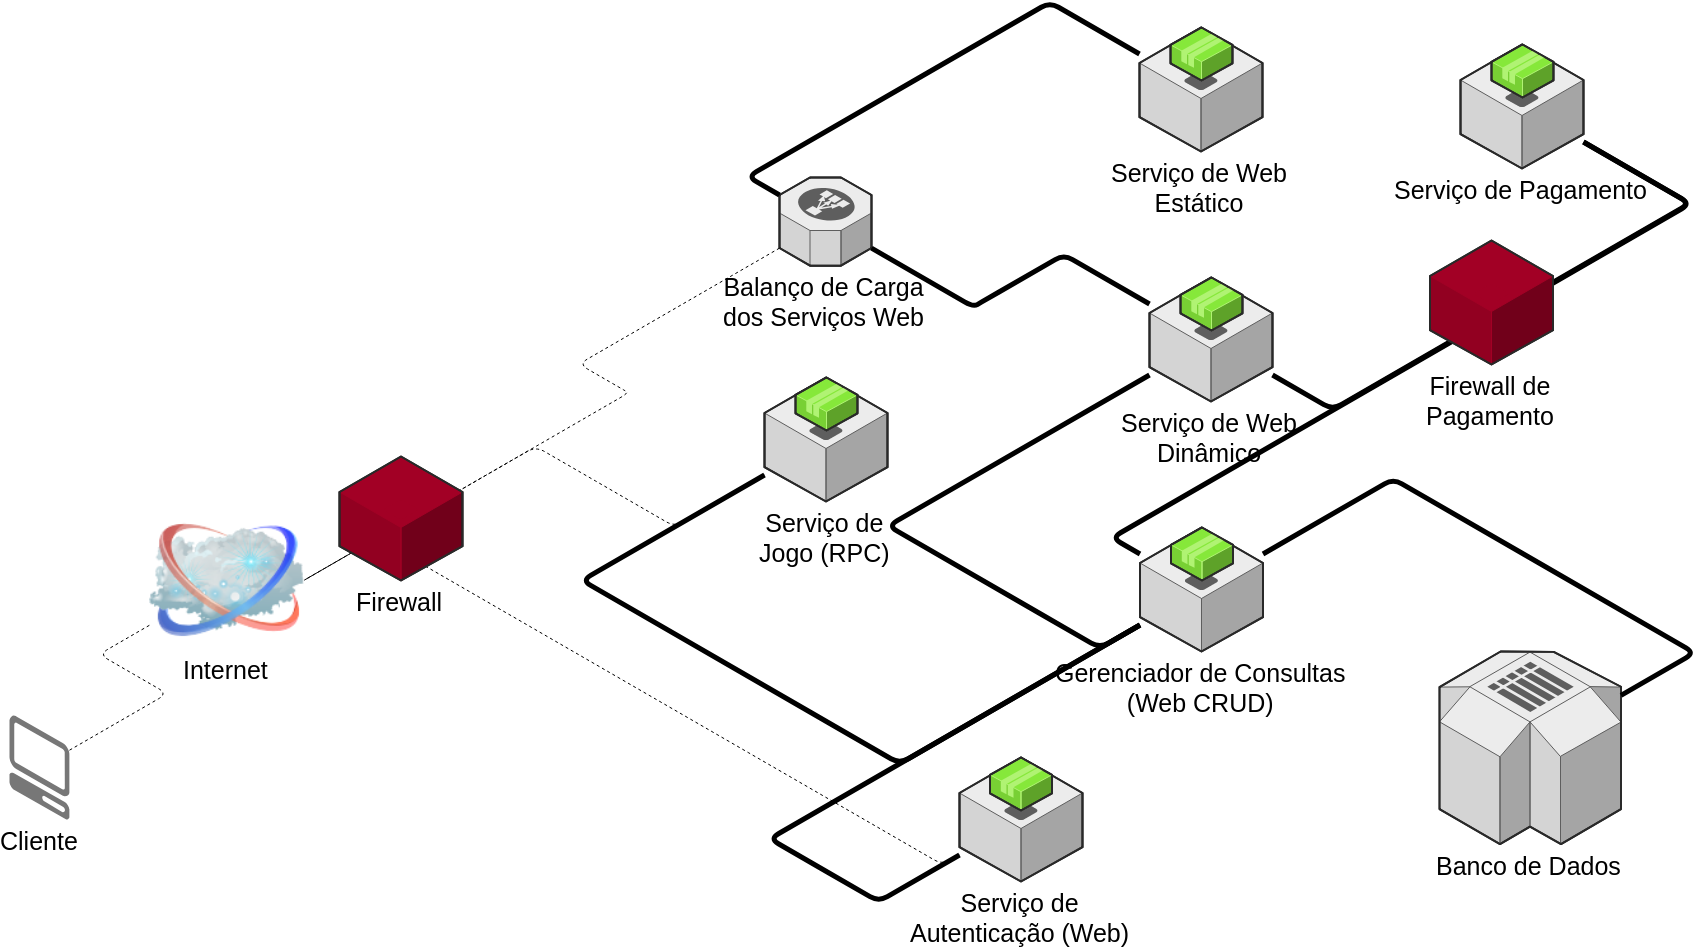
\includegraphics[height=5.5cm]{arquiteturas/full_rudy_fw.png}
  \centering

  Fonte:~\cite{matthiasrudy2011}.
\end{figure}




O funcionamento interno do serviço de jogo trabalha em rodadas, visando não penalizar usuários com baixa transferência de dados entre o cliente e o serviço.
%
Cada cliente produz requisições para ser consumido pelo ciclo de processamento do gerente de jogo. Entretanto o serviço irá consumir de forma igualitária uma requisição de um jogador diferente, como uma fila~\cite{albion_online_unite, matthiasrudy2011}.
%
O modelo de processamento do gerente de ambiente pode ser visualizado na Figura~\ref{fig:processamento}.



\begin{figure}[htb!]
  \caption{Modelo de \textit{Threads} do gerente de ambiente.}
  \label{fig:processamento}
  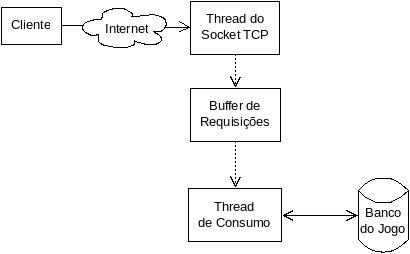
\includegraphics[height=4.5cm]{img/cap3/thread_model.png}
  \centering

  Adaptado de:~\cite{matthiasrudy2011} e ~\cite{albion_online_unite}.
\end{figure}

O mesmo modelo de processamento paralelo apresentado na Figura~\ref{fig:processamento} para consumo das requisições dos clientes é utilizado de forma similar na arquitetura Willson (Seção~\ref{willson}) e Salz (Seção~\ref{salz}).

Um serviço que chama atenção na arquitetura Rudy é o Gerenciador de Consultas, um serviço web que implementa uma camada sobre diversos bancos de dados a fim de prover variedade entre vários bancos de forma facilitada por requisições web, utilizando operações \ac{crud}.
%
Implementar esta camada garante uma padronização de acesso ao banco de dados, porém adiciona um possível gargalo a arquitetura~\cite{matthiasrudy2011}.

Os pontos positivos de utilizar esta camada de consultas na arquitetura é~\cite{matthiasrudy2011}:
\begin{enumerate}
  \item Não permite acesso direto ao banco de dados do serviço web e do serviço de jogo.
  \item Permite maior manejo a migrações em tabelas e troca de tecnologias.
  \item Define uma sintaxe estrita para consulta, via \ac{crud}.
  \item Permite acesso do banco a diversos serviços, sem gerenciar o banco.
  \item Permite contar número de requisições e tempo das requisições.
\end{enumerate}

Entretanto adicionando uma camada sobre os bancos de dados para gerenciamento tem pontos negativos~\cite{matthiasrudy2011}.

\begin{enumerate}
  \item Aumenta a complexidade de implementação, teste, administração e ponto de falha.
  \item Adiciona limites como número de conexões, número de requisições, etc.
\end{enumerate}



COMO LIGAR DUAS ARQUITETURAS?


\subsection{Arquitetura elaborada por Salz}
\label{salz}

A arquitetura elaborada por Salz~\cite{albion_online_unite}, a qual pode ser visualizada na Figura~\ref{full_salz} contém 7 microsserviços especializados para seu funcionamento.
%
Para o funcionamento adequado, o cliente necessita manter 3 conexões abertas com o servidor, sendo a conexão de jogo a com maior demanda~\cite{albion_online_unite}.

\begin{figure}[htb!]
  \caption{Arquitetura Salz completa.}
  \label{full_salz}
  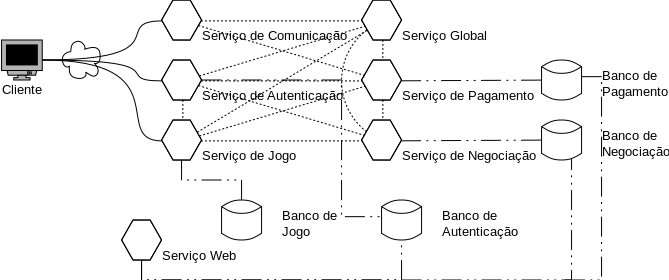
\includegraphics[height=5.5cm]{arquiteturas/full_salz.png}
  \centering

  Fonte:~\cite{albion_online_unite}.
\end{figure}

A Figura~\ref{full_salz} exibe a arquitetura salz de forma completa. Nela encontra-se 4 bancos de dados distintos, sendo eles banco de dados \ac{sql}, exceto ao banco de jogo, que utiliza um banco de \ac{nosql} com tecnologia chave-valor em memória.
%
Referente aos microsserviços que compõem a arquitetura, temos os seguintes elementos~\cite{salz_albion}:

\begin{enumerate}
  \item \textbf{Serviço de Comunicação}: Gerencia a troca de mensagens entre os jogadores. Opera sobre o protocolo \ac{rpc}.
  \item \textbf{Serviço de Autenticação}: Recepciona e gerencia as conexões dos clientes entre os demais microsserviços. Opera sobre o protocolo \ac{http}.
  \item \textbf{Serviço de Jogo}: Gerencia o estado do mundo, referente a um \textit{chunk} do ambiente. Opera sobre o protocolo \ac{rpc}.
  \item \textbf{Serviço Global}: Gerencia operações globais (\textit{e.g,} interações entre grupos, procedimentos recorrentes globais, \textit{etc.}). Opera sobre \ac{http}.
  \item \textbf{Serviço de Pagamento}: Efetua operações bancárias com serviços externos de pagamento e gerencia o estado de pagamento das contas. Opera sobre o protocolo \ac{https}.
  \item \textbf{Serviço de Negociação}: Opera como um serviço de leilão para itens do jogo. Opera sobre o protocolo \ac{http}.
\end{enumerate}


\subsection{Arquitetura elaborada por Willson}
\label{willson}



A arquitetura Willson~\cite{stephenclarkewillson2017} (Figura~\ref{fig:willson}) tenta suprir a necessidade de migração de conexão entre microsserviços ao personagem transladar dentre \textit{chunks} distintos.
%
Dessa forma, a arquitetura deixa de armazenar a estrutura da cena em memória para armazenar os status de objetos do ambiente em um banco de dados em memória compartilhado.
%
Nesse sentido, o ambiente torna-se escalável, porém é limitado ao desempenho do banco de dados escolhido.
%
Esta arquitetura permite implantar microsserviços sem configurações individuais, na qual facilita a sua gestão de manutenção e distribuição de carga.



\begin{figure}[htb!]
  \caption{Arquitetura Salz.}
  \label{fig:willson}
  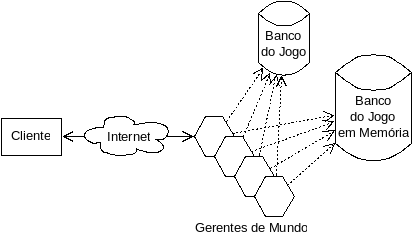
\includegraphics[height=4.5cm]{img/cap3/willson.png}
  \centering

  Adaptado de:~\cite{albion_online_unite}.
\end{figure}



O processamento de requisições segue o modelo de processamento paralelo descrito na Figura~\ref{fig:processamento}.
%
Entretanto, este serviço não armazenará nada em sua memória, realizando todas as operações no banco do jogo em memória.




A qualidade de serviço e custo de operação de serviços de jogos massivos é suscetível a arquitetura empregada.
%
Portanto, o embasamento técnico do funcionamento destas arquiteturas pode ajudar na definição de estratégias que diminuam o consumo de recursos e contribuam com a qualidade de serviço e custo ao usuário final, criando jogos mais competitivos no mercado.


\section{Definição do Problema}



A escolha de uma arquitetura para serviços \ac{mmorpg} que não suportem uma elevada carga de trabalho podem ser um eventual problema na escalabilidade do negócio de empresas que forneçam tais serviços.
%
Em alguns serviços, a divisão da carga é dada pela área de interesse, dividindo o ambiente em pedaços a fim de diminuir a carga no serviço.
%
Entretanto, locais populares no ambiente do jogo ainda são vulneráveis a disponibilidade de serviço~\cite{1417630}.



Nesse sentido, arquiteturas de microsserviços surgiram com o objetivo de aumentar a disponibilidade e viabilizar produtos de demanda massiva.
%
Tais arquiteturas dividem o seu funcionamento em módulos menores a fim de proporcionar maior demanda utilizando uma abordagem distribuída.
%
Entretanto, o custo de atender uma alta demanda de conexões pode consumir uma quantia de recursos computacionais ou uma qualidade insatisfatória de serviço, inviabilizando a sua utilização no mercado.



Um exemplo de implementação de arquitetura de um jogo \ac{mmorpg} pode ser visualizado na Figura~\ref{fig:generica}, no qual cada cliente deve conectar em um microsserviço de gerenciamento de mundo para receber as atualizações da região e submeter seus comandos.
%
Nessa arquitetura, é necessário levar em conta o funcionamento, método de compartilhamento dos dados e abordagem para processamento do ambiente do jogo a fim de descrever a sua escalabilidade e qualidade de serviço.


\begin{figure}[htb!]
\caption{Arquitetura de um jogo \ac{mmorpg} genérico.}
\label{fig:generica}
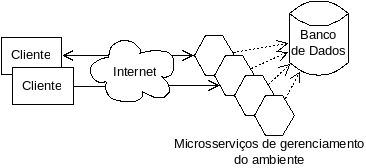
\includegraphics[height=6.0cm]{img/cap3/generica.png}
\centering

Fonte: O próprio autor
\end{figure}

A arquitetura genérica descrita na Figura~\ref{fig:generica} também precisa corresponder as demandas necessárias do \textit{GameDesign} do próprio jogo.
%
Neste caso, só um tipo de microsserviço é visível nesta rede, porém poderiam existir microsserviços responsáveis pela parte social, comércio e estatísticas, aumentando o grau de complexibilidade da arquitetura.
%
Em relação aos recursos utilizados por uma arquitetura, este trabalho foca na análise das arquiteturas de microsserviços descritas na literatura a fim de descrever o seu comportamento e desempenho.



A literatura aborda a previsibilidade de carga, análise de disponibilidade e uso de recurso de tais arquiteturas (a fim de guiar escolhas na etapa de \textit{Game Design} do produto e viabilizar o comércio do mesmo), relatados na Seção~\ref{sec:similares}.
%
Torna-se de interesse para empresas de desenvolvimento de jogos \ac{mmorpg} analisar o impacto e uso de recursos computacionais ao implantar uma arquitetura de microsserviços \ac{mmorpg} visando melhorar a disponibilidade de tais jogos.
%
Dentro do cenário de testes espera-se analisar por exemplo a estabilidade, limite de conexões e custo de processamento de tais arquiteturas.
%
Além disso, espera-se simular a carga de uma arquitetura utilizada em produção, a fim de possibilitar a quantificação do custo de operação de tal serviço.
%
Estas são expectativas gerais do que espera-se analisar, mas conforme a análise dos dados obtidos for realizada, é possível que outras características surjam.
%
Para guiar a proposta, um dos passos importantes são os trabalhos relacionados com este tema, na qual analisa-se estudos que abordam arquiteturas de jogos \ac{mmorpg} e/ou arquiteturas de microsserviços.



\section{Trabalhos Relacionados}
\label{sec:similares}



Para nortear o desenvolvimento da análise de microsserviços utilizados em jogos \ac{mmorpg} proposto no atual trabalho, essa seção apresenta outros trabalhos que têm o escopo ou objetivo similar, no qual monitoraram e analisaram serviços de jogos \ac{mmorpg}.
%
Ao apresentar estes trabalhos, busca-se apresentar o contexto e objetivo, e então aprofundar em características dos trabalhos, métricas utilizadas e ferramentas que auxiliaram nas análises.


Para encontrar os trabalhos relacionados, foi efetuada uma busca pelos termos \ac{mmorpg} ou \textit{microsservices}.
%
Entretanto, os dois termos dificilmente se correlacionam nos meios de busca disponíveis para a elaboração deste TCC.
%
Nesse sentido, os trabalhos relacionados abordam arquiteturas de jogos \ac{mmorpg} ou arquiteturas de microsserviços.



Como critério de análise, foi observado em questão qual a classificação em que o trabalho encontra-se, entre previsão de carga ou análise de arquitetura, e quais métricas foram utilizadas na análise.

\subsection{Huang et al. (2004)}
\label{sec:huang}



O trabalho de ~\cite{1417630} investiga a relação entre os recursos utilizados e o número de conexões presentes em um serviço \ac{mmorpg} distribuído.
%
Neste trabalho é relatado que a infraestrutura utiliza três serviços: Um \textit{Game Server} sobre protocolo \ac{tcp}, um \textit{Proxy Server} também sobre protocolo \ac{tcp}, e um servidor web para autenticação que executa sobre uma interface \ac{http}.
%
O foco de análise é o \textit{Proxy Server}, um serviço especificado em receber requisições e repassar atualizações da área de interesse destes jogadores, e o \textit{Game Server}, um serviço especificado para consumir as requisições realizadas pelo jogador.



\begin{figure}[htb!]
\caption{Arquitetura distribuída utilizando proxy.}
\label{fig:game_with_proxy}
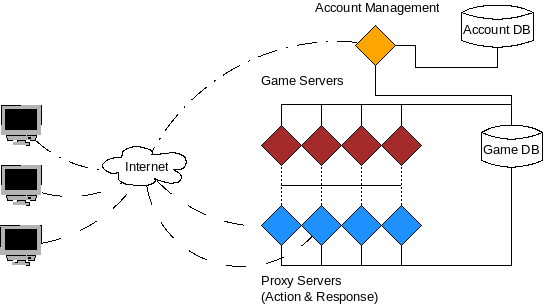
\includegraphics[height=7cm]{img/cap2/game_with_proxy.png}
\centering

Adaptado de:~\cite{1417630}.
\end{figure}



A infraestrutura do servidor de jogo contém um \textit{Proxy Server Farm} utilizando o algoritmo \textit{Round Robin} com pesos para balanceamento de carga entre cada cliente.
%
Cada \textit{Proxy Server} é responsável por comunicar com os demais microsserviços privados ao servidor, baseado com a área de interesse de sua conexão.
%
O protocolo de comunicação utilizado entre o Cliente e \textit{Proxy Server} é baseado em \ac{rpc}~\cite{faber, borella}, porém não é relatado sobre o o protocolo de comunicação utilizado entre o \textit{Proxy Server} e o \textit{Game Server}.
%
A sua arquitetura pode ser observada na Figura \ref{fig:game_with_proxy}, na qual obteve seus dados obtidos durante 100 dias para realizar as análises.
%
A Figura \ref{fig:players_peer_time} demonstra uma amostra do número de conexões pelo tempo no serviço obtido.



\begin{figure}[htb!]
\caption{Número de conexões no serviço pelo tempo decorrido.}
\label{fig:players_peer_time}
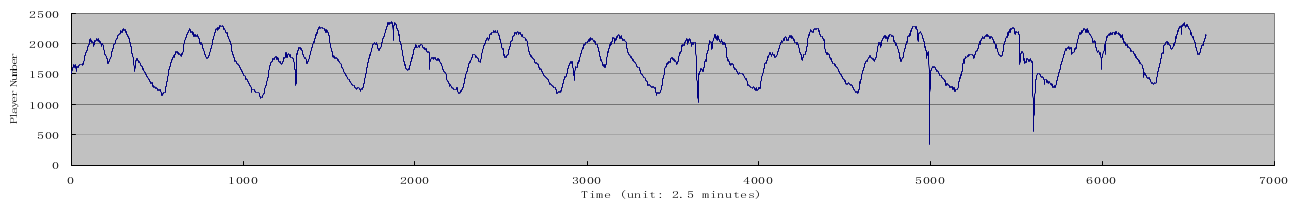
\includegraphics[height=2.5cm]{img/cap2/players_peer_time.png}
\centering

Fonte:~\cite{1417630}.
\end{figure}



Como análise, o autor correlacionou o número de conexões com número de pacotes e banda, consumidos, utilizando uma função estatística linear.
%
Esta função pode ser utilizada com regressão linear para prever consumo de recursos futuros e por fim realocar mais recursos ao serviço, contribuindo com escalabilidade vertical autônoma.
%
Um exemplo de aplicação dessa regressão linear pode ser visualizada na Figura~\ref{fig:regressao_bytes}, no qual o autor compara o consumo de banda real comparado a regressão linear.



\begin{figure}[htb!]
\caption{Regressão linear comparado ao consumo de banda real do servidor.}
\label{fig:regressao_bytes}
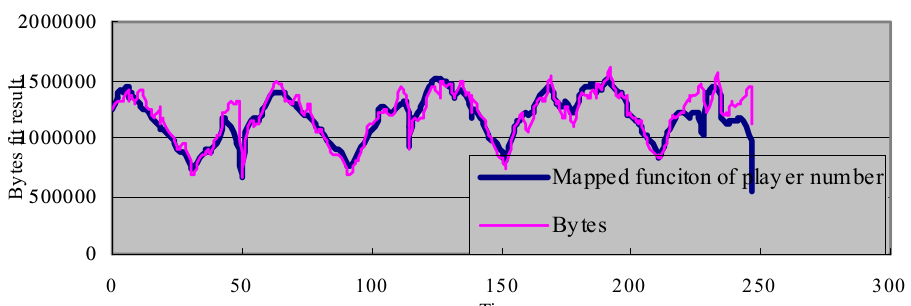
\includegraphics[height=4.5cm]{img/cap2/regressao.png}
\centering

Fonte:~\cite{1417630}
\end{figure}



Entretanto, a escalabilidade horizontal não pode ser prevista, visto que não é analisado o posicionamento de cada personagem a fim de dividir os ambientes em pedaços menores com outros serviços.
%
Como trabalhos futuros é relatado a análise do posicionamento de personagens para escalabilidade horizontal, a análise de outras arquiteturas e a análise de outros gêneros de jogos, além do impacto de utilizar balanço de carga e provisionamento de recursos de forma dinâmica.



\subsection{Villamizar et al. (2016)}



O trabalho de ~\cite{7515686} investiga o custo de arquiteturas de microsserviços, arquiteturas \ac{paas} orientadas a eventos e aplicações monolíticas para aplicações web.
%
A sua principal motivação é a comparação de custos para a tradução de sistemas legados para arquiteturas distribuídas.
%
Para isso, o autor preparou três instâncias de testes com suas configurações desenhadas a fim de ter o maior número de requisições por minuto com o mesmo custo financeiro.



\begin{figure}[htb!]
\caption{Arquitetura monolítica web implementada na \ac{aws}}
\label{fig:aws_monolitico}
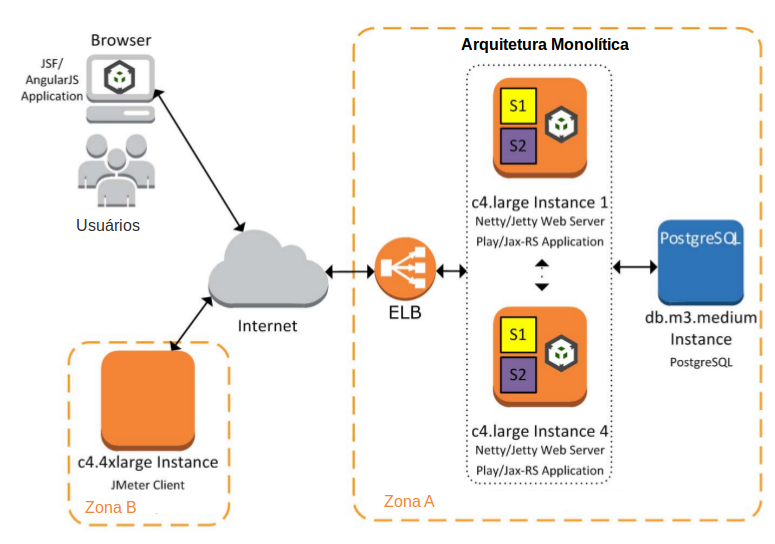
\includegraphics[height=6.5cm]{img/cap2/aws_monolitico.png}
\centering

Fonte:~\cite{7515686}
\end{figure}
%ccm Figura em português


\textbf{Instância I.} Utilizando quatro instâncias \ac{aws} \textit{c4.large}, uma instância \ac{aws} \textit{c4.xlarge} e uma instância \ac{aws} \textit{db.m3.medium}.
%
A Figura~\ref{fig:aws_monolitico} exibe a implantação de uma aplicação web monolítica.
%
Essa arquitetura foi implementada utilizando \textit{Jax-RS} e \textit{Play Framework}.




\begin{figure}[htb!]
\caption{Arquitetura de microsserviços web implementada na \ac{aws}}
\label{fig:aws_microsservicos}
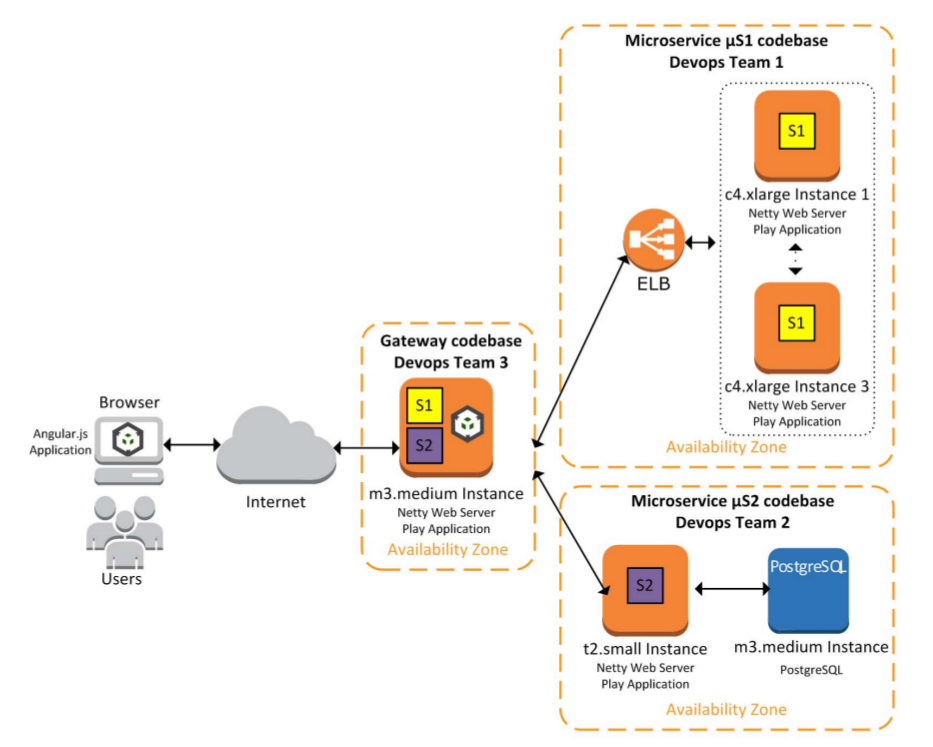
\includegraphics[height=6.5cm]{img/cap2/aws_microsservicos.png}
\centering

Fonte:~\cite{7515686}
\end{figure}
%ccm Figura em português

\textbf{Instância II.} Utilizando três instâncias \ac{aws} \textit{c4.xlarge}, uma instância \ac{aws} \textit{t2.small} e uma instância \ac{aws} \textit{db.m3.medium}.
%
A Figura~\ref{fig:aws_microsservicos} exibe a implantação de uma aplicação de microsserviços web. Essa arquitetura foi implementada utilizando \textit{Play Framework}. %ccm <-14



\begin{figure}[htb!]
\caption{Arquitetura de microsserviços web implementada na \ac{aws} utilizando a tecnologia \textit{lambda}}
\label{fig:aws_lambda}
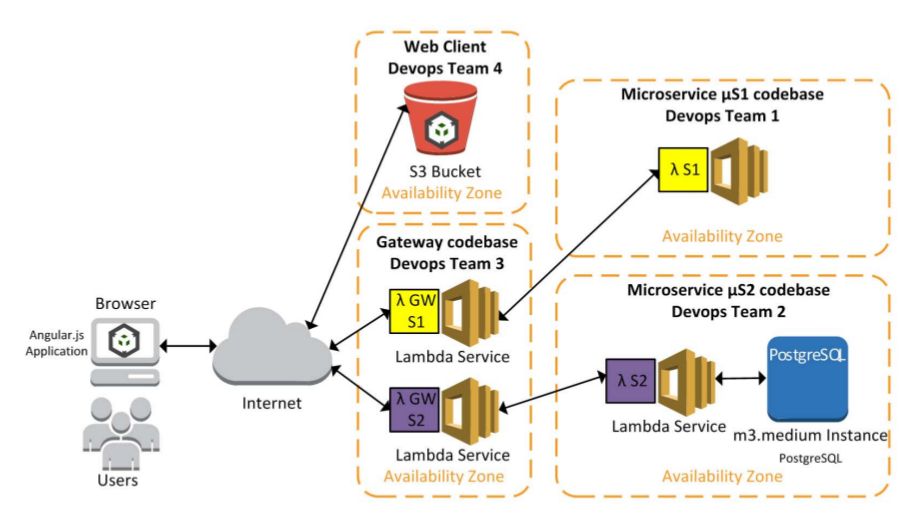
\includegraphics[height=6.5cm]{img/cap2/aws_lambda.png}
\centering

Fonte:~\cite{7515686}
\end{figure}
%ccm Figura em português

\textbf{Instância III.} Utilizando duas instâncias \ac{aws} \textit{lambda S1}, duas instâncias \ac{aws} \textit{lambda S2}, uma instância \ac{aws} \textit{S3 Bucket} e uma instância \ac{aws} \textit{db.m3.medium}.
%
A Figura~\ref{fig:aws_lambda} exibe a implantação de uma aplicação de microsserviços web utilizando a tecnologia \ac{aws} \textit{lambda}. Essa arquitetura foi implementada em \textit{Node.js}, nas quais as funções de \textit{gateway} foram implementadas em quatro funções independentes do tipo \textit{microservice-http-endpoint}. %ccm <-39



\begin{figure}[htb!]
\caption{Custo por um milhão de requisições em dólares utilizando diferentes arquiteturas sobre a \ac{aws}}
\label{fig:custo_aws}
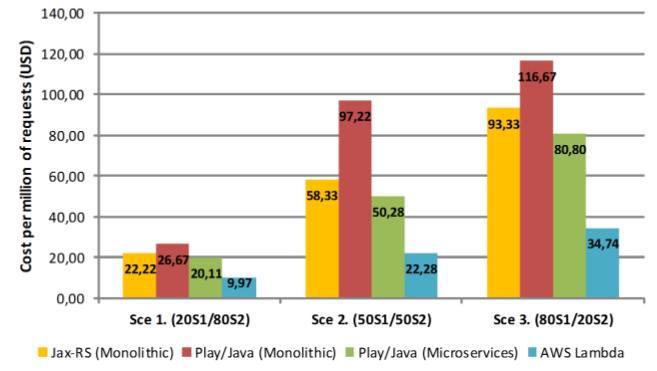
\includegraphics[height=6.5cm]{img/cap2/custo_aws.png}
\centering

Fonte:~\cite{7515686}
\end{figure}



Foi concluído que a arquitetura de microsserviços, nas condições desta aplicação, podem reduzir até 13.42\% em gastos com a infraestrutura.
%
Essa redução pode ser observada na Figura~\ref{fig:custo_aws}.
%
O autor alerta sobre tolerância a falhas, transações distribuídas, distribuição de dados e versionamento de serviço.


\subsection{Suznjevic e Matijasevic (2012)}



O trabalho de ~\cite{6374456} tem seu objetivo a fim de prever a carga a qual um serviço \ac{mmorpg} pode receber utilizando a complexidade das operações nos contextos de \ac{pvp} e \ac{pvnpc} a qual um personagem pode realizar em um ambiente.
%
Este trabalho usa com base o modelo descrito na Seção~\ref{sec:huang}, um modelo distribuído em serviços na qual efetuam o processamento de uma região do ambiente virtual.



\begin{table}[htb!]
\centering
\caption{Complexidade da interação com o ambiente, por contexto da interação}
\label{tab:complexidade}
\begin{tabular}{|l|l|l|l|l|}
\hline
Contexto da ação        & \ac{pvp}           & \ac{pvnpc}              & Número de \ac{npcs}    & Network {[}kbits/s{]} \\ \hline
Questing                & $O(n)$             & $O(n log(n))$           & $N \leq 6 $            & 11.4          \\ \hline
Trading                 & $O(n)$             & $O(n)$                  & $N \leq 20$            & 8.1           \\ \hline
Dungeons                & $O(n^2)$           & $O(n^2)$                & $N \leq 20$            & 18.3          \\ \hline
\ac{pvp} combat         & $O(n^3)$           & $O(n)$                  & $N = 0    $            & 24.1          \\ \hline
Raiding                 & $O(n^2 log(n))$    & $O(n^3)$                & $N \leq 40$            & 32.0          \\ \hline
\end{tabular}

Fonte:~\cite{6374456}
\end{table}
%ccm traduzir


A análise realizada leva em conta a complexidade das ações no ambiente, a qual pode ser descrita na Tabela~\ref{tab:complexidade}.
%
Essa tabela exibe as ações que podem ser executadas para interagir com o ambiente, seja essa interação com \ac{pvp} (jogador com outro jogador) ou \ac{pvnpc} (jogador com um personagem ou objeto gerenciado pelo serviço).
%
Os contextos analisados nessa tabela são:

\begin{itemize}
  \item \textit{Questing}: Contexto de missão, na qual um grupo de jogadores ou um grupo de \ac{npcs} podem ser afetados nas ações.
  \item \textit{Trading}: Contexto de negociação, na qual a complexidade leva em conta somente o número de itens negociados.
  \item \textit{Dungeons}: Contexto de exploração, na qual o ambiente pode ser modificado conforme as ações dos personagens em um ambiente isolado para este grupo.
  \item \textit{\ac{pvp} combat}: Contexto de batalha entre jogadores, na qual as ações entre os jogadores influenciam diretamente o estado do personagem oponente.
  \item \textit{Raiding}: Representa um contexto específico de exploração, na qual múltiplos jogadores unem forças a fim de combater outro grupo de jogadores ou \ac{npcs}.
\end{itemize}


\begin{figure}[htb!]
\caption{Regressão levando em conta a complexidade das ações e contexto dos personagens}
\label{fig:regressao_complexidade}
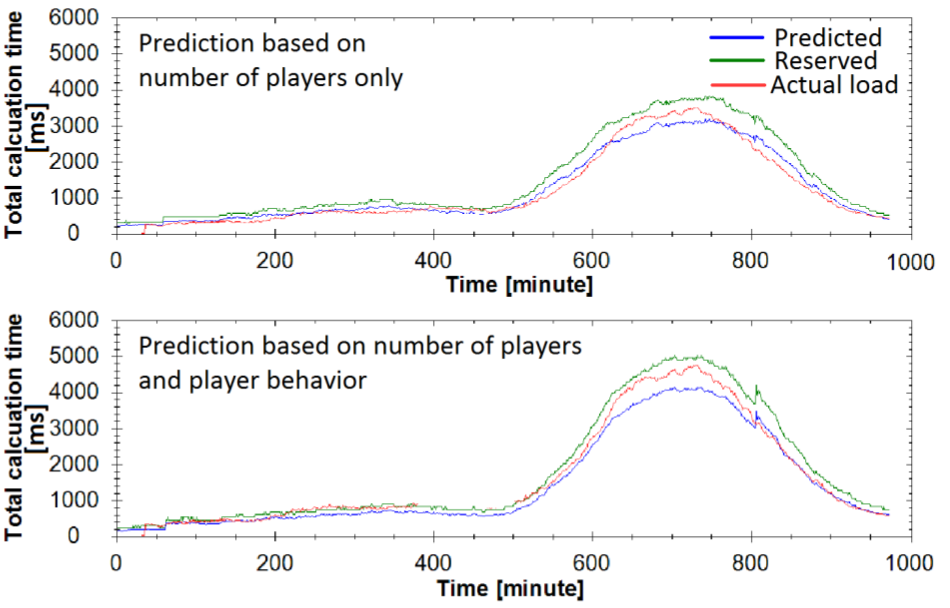
\includegraphics[height=6.0cm]{img/cap2/network_regressao_complexidade.png}
\centering

Fonte:~\cite{6374456}
\end{figure}
%ccm Figura em português


Utilizando as complexidades das ações, o número de conexões e o contexto de cada personagem no ambiente para predizer a banda utilizada.
%
Pode-se visualizar uma regressão na Figura~\ref{fig:regressao_complexidade}.



O autor conclui que o contexto de interação com o ambiente de cada personagem tem relevância com o consumo de \ac{cpu} e banda, a qual pode ser calculada com sua complexidade a fim de desenvolver uma ferramenta para predição de carga sobre serviços \ac{mmorpg}.
%
Entretanto, essa predição não é feita em tempo real, não contribuindo para a automação da escalabilidade vertical e horizontal da arquitetura de microsserviços.



\subsection{Análise dos trabalhos relacionados}
\label{sec:similares_analise}



%Em específico, nesta seção são apontadas características relevantes a cada trabalho e por fim é feita uma comparação entre estas características. %ccm <- Melhorar
%
Ao levantar o problema de consumo de recursos, existem duas vertentes de pesquisas, sendo descritas dessa forma: %ccm <-8

\begin{itemize}
  \item \textbf{Comparação de arquiteturas}: O autor utiliza alguma métrica a fim de decidir qual a melhor alternativa de arquitetura para determinada aplicação.
  \item \textbf{Previsão de carga}: Projetar a carga futura sobre algum recurso a fim de escalar automaticamente a sua arquitetura na nuvem, a fim de reduzir gastos de alocações ociosas.
\end{itemize}

Dessa forma, pode-se dividir os trabalhos relacionados com a sua categoria.
%
Esta relação pode ser visualizada na Tabela~\ref{tab:categoria_trabalhos}.

\begin{table}[htb!]
\centering
\caption{Trabalhos relacionados por categoria}
\label{tab:categoria_trabalhos}
\begin{tabular}{|l|l|}
\hline
Autor & Categoria                            \\ \hline
\cite{6374456}  & Previsão de carga          \\ \hline
\cite{7515686}  & Comparação de arquiteturas \\ \hline
\cite{1417630}  & Previsão de carga          \\ \hline
\end{tabular}


Fonte: O próprio autor.
\end{table}

Para o trabalho referente a comparação de arquiteturas~\cite{7515686}, o recurso utilizado foi o custo por um determinado número de requisições web.
%
Já para os trabalhos referentes a previsão de carga~\cite{6374456, 1417630} foi levantado o consumo da banda, \ac{cpu} e memória, entretanto não levantou-se o número de conexões e latência aos usuários, na qual podem ser observados na Tabela~\ref{tab:recursos_categoria}.
%
Nenhum trabalho relatou limite de conexões ou latência do sistema.

\begin{table}[htb!]
\centering
\begin{adjustbox}{max width=\textwidth}
\caption{Trabalhos relacionados por recurso utilizado}
\label{tab:recursos_categoria}
\begin{tabular}{|l|l|l|l|l|l|l|l|}
\hline
Autor           & \ac{cpu}   & Memória    & Banda      & Custo      & Latência & \makecell{Limite \\ de \\ conexões} & \makecell{Complexidade \\ de \\ Algoritmos} \\ \hline
\cite{1417630}  & $\times$   & $\times$   & \checkmark & $\times$   & $\times$ & $\times$                            & $\times$                                    \\ \hline
\cite{7515686}  & $\times$   & $\times$   & $\times$   & \checkmark & $\times$ & $\times$                            & $\times$                                    \\ \hline
\cite{6374456}  & \checkmark & \checkmark & \checkmark & $\times$   & $\times$ & $\times$                            & \checkmark                                  \\ \hline
\end{tabular}
\end{adjustbox}

Fonte: O próprio autor.
\end{table}



Outro ponto a ser analisado são as arquiteturas utilizadas. Os trabalhos referentes a previsão de carga não utilizaram uma arquitetura de microsserviços, mesmo sendo um sistema distribuído.
%
Nesses serviços, os sistemas eram dependentes entre sí e precisavam um dos outros para o seu funcionamento.
%
A relação de arquiteturas abordadas pode ser visualizado na Tabela~\ref{tab:arquiteturas_analisadas}, na qual mostra quais trabalhos abordaram os temas sobre arquiteturas de microsserviços e jogos \ac{mmorpg}.
%
Além disso, não foi descrito um método de replicação automática dos serviços a fim de prover alta disponibilidade de forma automatizada, sendo abordado como um trabalho futuro.


\begin{table}[htb!]
\centering
\begin{adjustbox}{max width=\textwidth}
\caption{Arquiteturas Analisadas}
\label{tab:arquiteturas_analisadas}
\begin{tabular}{|l|l|l|l|}
\hline
Autor           & Arquitetura de Microsserviços & Arquitetura Distribuída  & \ac{mmorpg}   \\ \hline
\cite{1417630}  & $\times$                      & \checkmark               & \checkmark    \\ \hline
\cite{7515686}  & \checkmark                    & \checkmark               & $\times$      \\ \hline
\cite{6374456}  & $\times$                      & \checkmark               & \checkmark    \\ \hline
\end{tabular}
\end{adjustbox}

Fonte: O próprio autor.
\end{table}


Este Trabalho de Conclusão de Curso pretende analisar uma arquitetura de microsserviços especificada a jogos \ac{mmorpg}, visando métricas de desempenho e custo de operação. %ccm <-11
%ccm defnir métricas

\section{Considerações parciais}

Este capítulo conceituou jogos eletrônicos, gênero de jogo e especificou as características de um jogo \ac{mmorpg}.
%
Após apresentar sobre o gênero de jogo abordado, detalha-se a sua jogabilidade, problemas relevantes a este gênero do ponto de vista de rede de computadores e por fim sobre técnicas e abordagens populares acerca do desenvolvimento destes serviços, a qual serão utilizados no problema deste Trabalho de Conclusão de Curso.


Por fim, são apresentados trabalhos relacionados a fim de guiar por métricas, métodos de coleta de dados e métodos de desenvolvimento e implantação de tais arquiteturas a fim de contribuir com o atual escopo do trabalho.
%
Entretanto, houve uma dificuldade em encontrar na literatura analises sobre arquiteturas de microsserviços focado a jogos, principalmente em específico o gênero \ac{mmorpg}.
%
Dessa forma, espera-se introduzir a analise da viabilidade e do custo de recursos computacionais para manter um serviço \ac{mmorpg} sobre uma arquitetura de microsserviços.
